
%%%%%%%%%%%%%%%%%%%%%%% file typeinst.tex %%%%%%%%%%%%%%%%%%%%%%%%%
%
% This is the LaTeX source for the instructions to authors using
% the LaTeX document class 'llncs.cls' for contributions to
% the Lecture Notes in Computer Sciences series.
% http://www.springer.com/lncs       Springer Heidelberg 2006/05/04
%
% It may be used as a template for your own input - copy it
% to a new file with a new name and use it as the basis
% for your article.
%
% NB: the document class 'llncs' has its own and detailed documentation, see
% ftp://ftp.springer.de/data/pubftp/pub/tex/latex/llncs/latex2e/llncsdoc.pdf
%
%%%%%%%%%%%%%%%%%%%%%%%%%%%%%%%%%%%%%%%%%%%%%%%%%%%%%%%%%%%%%%%%%%%


\documentclass[runningheads,a4paper]{llncs}

\usepackage{amssymb}
\setcounter{tocdepth}{3}
\usepackage{graphicx}
\usepackage{multirow}
\usepackage{subfigure}
\usepackage{graphics}
\usepackage{longtable}
\usepackage{rotating}
\usepackage{verbatim}
\usepackage{float}
%\usepackage[backend=bibtex8]{biblatex}
\usepackage{pbox}

\usepackage{url}
\urldef{\mailsa}\path|{alfred.hofmann, ursula.barth, ingrid.haas, frank.holzwarth,|
\urldef{\mailsb}\path|anna.kramer, leonie.kunz, christine.reiss, nicole.sator,|
\urldef{\mailsc}\path|erika.siebert-cole, peter.strasser, lncs}@springer.com|    
\newcommand{\keywords}[1]{\par\addvspace\baselineskip
\noindent\keywordname\enspace\ignorespaces#1}

\usepackage{listings}
\usepackage{color}
\definecolor{javared}{rgb}{0.6,0,0} % for strings
\definecolor{javagreen}{rgb}{0.25,0.5,0.35} % comments
\definecolor{javapurple}{rgb}{0.5,0,0.35} % keywords
\definecolor{javadocblue}{rgb}{0.25,0.35,0.75} % javadoc
 
\lstset{language=Java,
basicstyle=\ttfamily,
keywordstyle=\color{javapurple}\bfseries,
stringstyle=\color{javared},
commentstyle=\color{javagreen},
morecomment=[s][\color{javadocblue}]{/**}{*/},
%numbers=left,
numberstyle=\tiny\color{black},
stepnumber=2,
numbersep=10pt,
tabsize=4,
showspaces=false,
showstringspaces=false}

\def\rot{\rotatebox}





\begin{document}

\mainmatter  % start of an individual contribution

% first the title is needed
\title{Evaluation of ADFD and ADFD$^+$ techniques}

% a short form should be given in case it is too long for the running head
\titlerunning{Evaluation of ADFD and ADFD$^+$ techniques}

% the name(s) of the author(s) follow(s) next
%
% NB: Chinese authors should write their first names(s) in front of
% their surnames. This ensures that the names appear correctly in
% the running heads and the author index.
%
\author{Mian Asbat Ahmad%
%\thanks{Please note that the LNCS Editorial assumes that all authors have usedn the western naming convention, with given names preceding surnames. This determines the structure of the names in the running heads and the author index.}%
\and Manuel Oriol}
%
\authorrunning{Evaluation of ADFD and ADFD$^+$ techniques} %: Authors' Instructions}
% (feature abused for this document to repeat the title also on left hand pages)

% the affiliations are given next; don't give your e-mail address
% unless you accept that it will be published
\institute{University of York, Department of Computer Science,\\
Deramore Lane, YO10 5GH YORK, United Kingdom\\
%\mailsa\\
%\mailsb\\
%\mailsc\\
%\url{http://www.springer.com/lncs}}
}

%
% NB: a more complex sample for affiliations and the mapping to the
% corresponding authors can be found in the file "llncs.dem"
% (search for the string "\mainmatter" where a contribution starts).
% "llncs.dem" accompanies the document class "llncs.cls".
%

\toctitle{Lecture Notes in Computer Science}
\tocauthor{Authors' Instructions}
\maketitle





\begin{abstract}

The ever-increasing reliance on software-intensive system is driving research to discover software faults more efficiently. Despite intensive research, very few approaches have studied and used knowledge about fault domains to improve the testing or the feedback given to developers. The shortcoming was addressed by developing ADFD and ADFD$^+$ strategies presented in our previous publications. In the present study, the two strategies were enhanced by integration of the automatic testing tool Daikon and the precision of identifying failure domains was determined through extensive experimental evaluation of real world Java projects contained in Qualitas Corpus. The analyses of results, cross-checked by manual testing indicated that ADFD and ADFD$^+$ techniques are highly effective in providing assistance but are not an alternative to manual testing with the limited available resources.


%The achievement of up-to 50\% better results by Adaptive Random Testing (ART) in comparison with Random Testing (RT) ensures that failure-domains within the input domain are useful and need due consideration in selection of test inputs. Our previously developed two automated techniques (ADFD and ADFD$^+$), automatically find failure and its domain in a specific range and present it graphically.
%They can precisely detect the failure-domain of the identified failure in an effective way. Performing exhaustive testing in a limited region around the failure is the key to the success of ADFD and ADFD+ techniques.

%In this article, we performed an extensive experimental analysis of Java projects contained in Qualitas Corpus for finding the effectiveness of automated techniques (ADFD and ADFD$^+$). The results obtained were analysed and cross-checked using manual testing. The impact of nature, location, size, type and complexity of failure-domains on the testing techniques were studied. The results provide insights into the effectiveness of automated techniques and a number of lessons for testing researchers and practitioners.

%The abstract should summarize the contents of the paper and shouldcontain at least 70 and at most 150 words. It should be written using the \emph{abstract} environment.
%\keywords{We would like to encourage you to list your keywords within the abstract section}
\keywords{software testing, automated random testing, manual testing, ADFD, ADFD$^+$, Daikon}

\end{abstract}




\section{Introduction}
The input-domain of a given System Under Test (SUT) can be divided into two sub-domains. The pass-domain comprises of the values for which the software behaves correctly and the failure-domain comprises of the values for which the software behaves incorrectly. Chan et al.~\cite{chan1996proportional} observed that input inducing failures are contiguous and form certain geometrical shapes. They divided these into point, block and strip failure-domains as shown in Figure~\ref{fig:patterns}. Adaptive Random Testing achieved up to 50\% better performance than random testing by taking into consideration the presence of failure-domains while selecting the test input~\cite{Chen2008}.

\smallskip
\begin{figure} [H]
\centering
\subfigure[Point domain]{
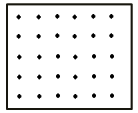
\includegraphics[width=2.5cm,height=2cm]{point.png}
\label{fig:point}
}
\subfigure[Block domain]{
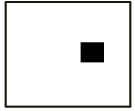
\includegraphics[width=2.5cm,height=2cm]{block.png}
\label{fig:block}
}
\subfigure[Strip domain]{
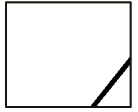
\includegraphics[width=2.5cm,height=2cm]{strip.png}
\label{fig:strip}
}
\smallskip
\caption{Failure domains across input domain~\cite{chan1996proportional}}
\label{fig:patterns}
\end{figure} 

%Adaptive Random Testing (ART) exploited the existence of the failure-domains and resultantly achieved up to 50\% better performance than random testing~\cite{Chen2008}. This was mainly attributed to the better distribution of input which increased the chance of selecting inputs from failure-domains. This insight motivated us to increase our understanding of failure-domains in production software.

%The cost of software testing constitute about half of the total cost of software development~\cite{myers2011art}. Software testing is an expensive but essential process which is particularly time consuming, laborious and error-prone when performed manually. Alternatively, automated software testing may involve higher initial cost but brings the key benefits of lower cost of production, higher productivity, maximum availability, greater reliability, better performance and ultimately proves highly beneficial for any organisation~\cite{Beizer1990}. A case study conducted by Pacheco et al. reveals that the 150 hours of automated testing found more faults in complex .NET code than a test engineer finds in one year by manual testing~\cite{pacheco2008finding}.

We have developed two fully automated techniques ADFD~\cite{ahmad2013adfd} and ADFD$^+$~\cite{ahmad2014adfd2}, which effectively find failures and failure domains in a specified range and also provide visualisation of the pass and fail domains. The process is accomplished in two steps. In the first step, an upgraded random testing is used to find the failure. In the second step, exhaustive testing is performed in a limited region around the detected failure in order to identify the domains. The ADFD searches in one-dimension and covers longer range than ADFD$^+$ which is more effective in multi-dimension and covers shorter range. Three separate tools including York Extensible Testing Infrastructure (YETI), Daikon and JFreeChart have been used in combination for developing ADFD and ADFD$^+$ techniques. The YETI~\cite{Oriol2011yeti}, Daikon~\cite{ernst2007daikon} and JFreeChart~\cite{gilbert2008jfreechart} are used for testing the program, generating invariants and plotting the pass and fail domains respectively.



%Software testing can be performed either automatically or manually. Both the techniques have their own advantages and limitations. The main advantage of automated testing is execution of large number of tests in little time, whereas manual testing utilizes the tester experience to concentrate on error-prone part of the SUT and generate target oriented test cases~\cite{Leitner2007}. 

%The analysis of failures and failure-domains discovered in 57 classes from 25 open source Java projects of Qualitas Corpus through three different techniques---ADFD, ADFD+ and Manual testing---reveals that each is good at uncovering different type of failure-domains and each brings distinct contributions.


The rest of the paper is organized as follows: \S~2 presents enhancement of the techniques. \S~3 shows the difference in working mechanism of the two techniques by a motivating example. \S~4 highlights the key research questions. \S~5 describes the evaluation process comprising experiments, results and answers to the research questions. \S~6 presents threats to validity while \S~7 points out the related work. Finally, \S~8 presents conclusion of the study.


 

%%%%%%%%%%%%%%%%%    ADFD and ADFD+   %%%%%%%%%%%%%%%%%%%

%\section{Automated Techniques}
%The two automated techniques used in our experiments are ADFD and ADFD+. A short overview of both the techniques and the enhancements that have been made to the techniques along with a motivating example are given below:

%\subsection{Overview of ADFD technique}
%Automated Discovery of Failure Domain is an automated technique for finding and drawing the failure domain of detected failure in the input domain. ADFD searches for failure domain between the specified lower and upper bound in uni-direction. It test and note only the ranges of pass and fail values and uses the scatter graph of the JFreeChart to plot them on the screen. For more details please see \cite{ahmad2013adfd}.

%\subsection{Overview of ADFD+ technique}
%Automated Discovery of Failure Domain+ is an automated technique for finding and drawing the failure domain of detected failure in the input domain. ADFD+ searches for failure domain around the failure in specified range in multi-idirection. It test and note individual value as either pass or fail. The values are drawn using the vector graph of the JFreeChart. For more details please see \cite{ahmad2014adfd2}.


\section{Enhancement of the techniques}
Prior to experimental evaluation, new features were incorporated in ADFD and ADFD$^+$ techniques to: increase the code coverage, provide information about the identified failure and generate invariants of the detected failure domains as stated below: 
\begin{enumerate}

\item The GUI was enabled to launch all the strategies defined in YETI from a single interface. As an example, if ADFD strategy is selected for testing, the system automatically hides the field (range value) associated with ADFD$^+$ and displays two fields of lower and upper bounds. On the other hand if ADFD$^+$ strategy is selected for testing, the system automatically hides the two fields (lower and upper bounds) associated with ADFD technique and displays a single field of range value.

\item Code coverage was increased by extending the techniques to support the testing of methods with \verb+byte, short, long, double+ and \verb+float+ type arguments while it was restricted to \verb+int+ type arguments only in the original techniques.

\item Invariants of the detected failure domains were automatically generated by integrating the tool Daikon in the two techniques. Daikon is an automated invariant detector that detects likely invariants in the program~\cite{ernst2007daikon}. The generated invariants are displayed in GUI at the end of test execution. 

\item The screen capture button was added to the GUI to allow the user to capture multiple screen-shots at different intervals of testing for future reference. 

\end{enumerate}

%\item Additional information was facilitated by adding the YETI generated failure finding test case to the GUI of the two techniques. Test case included type of failure, name of the failing class, name of the failing method, values causing the failure and line number of the code causing failure.


%\begin{figure}
%\centering
% \makebox[\textwidth][c]{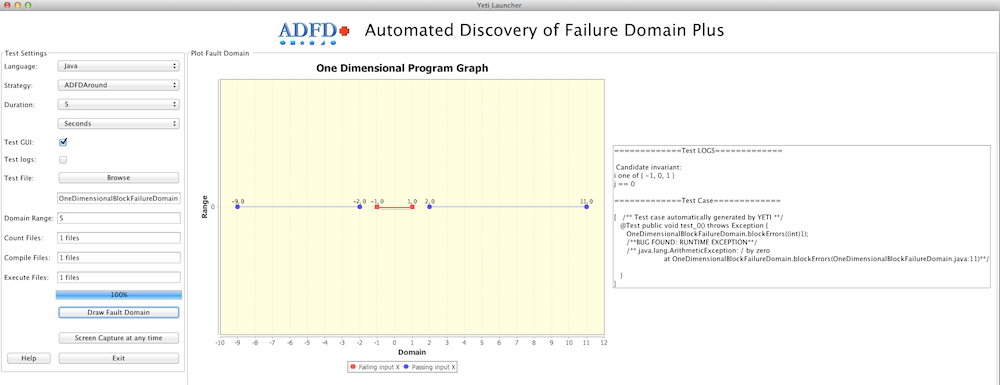
\includegraphics[width=1.25\textwidth, height=10cm]{chapter7/adfdUpgraded1.png}}%
% \bigskip
%  \caption{GUI front end of upgraded ADFD and ADFD$^+$}
%  \label{fig:adfdUpgraded}
%\end{figure}
%\bigskip
%\bigskip


%\begin{figure}[ht]

%\centering
%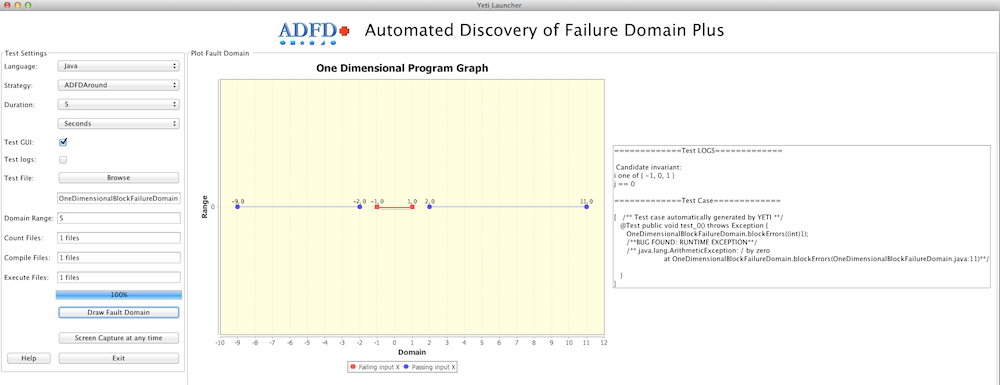
\includegraphics[width= 17.5cm,height=11cm]{chapter7/adfdUpgraded1.png}
%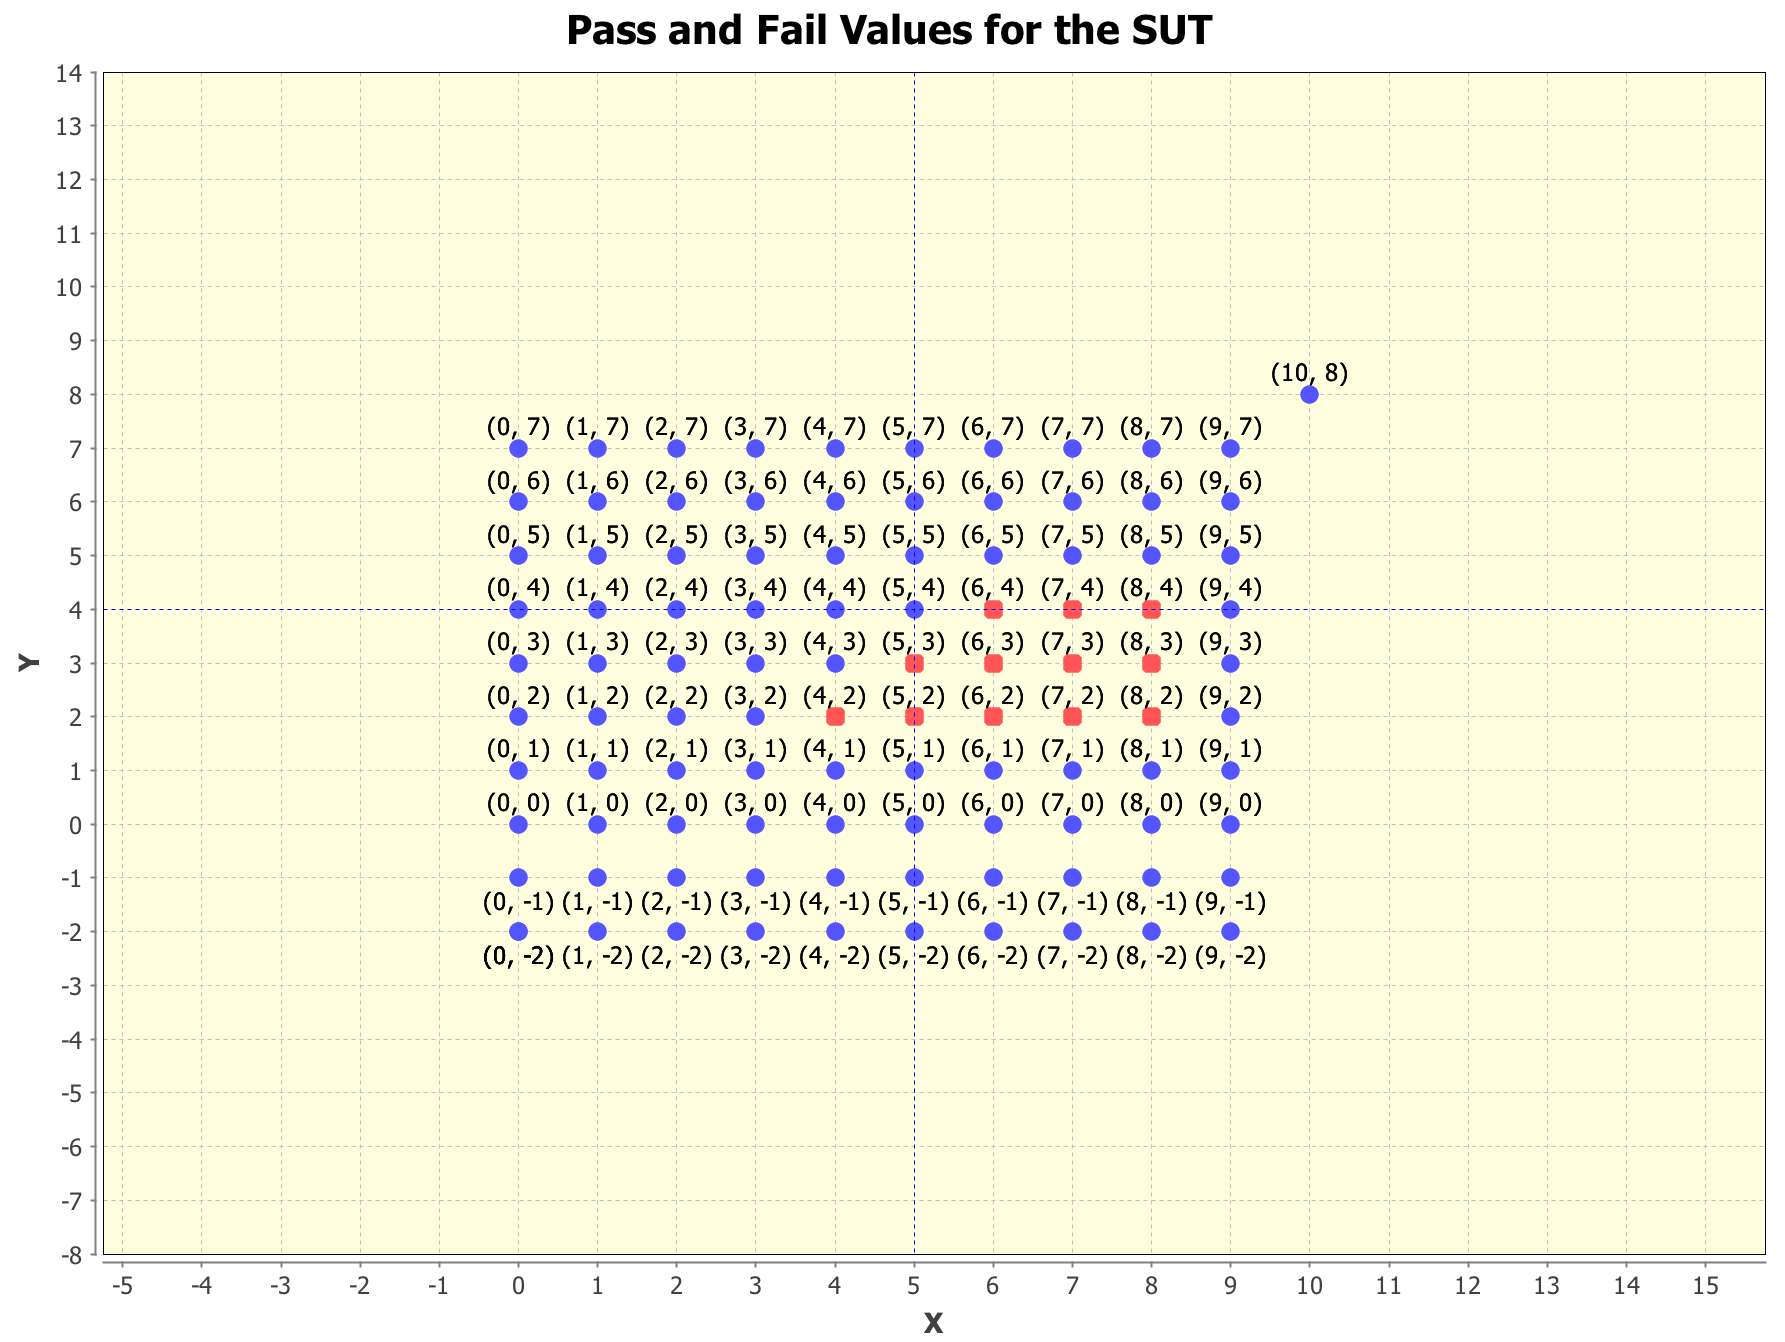
\includegraphics[width= 8.5cm,height=7cm]{adfdPlus1.png}
%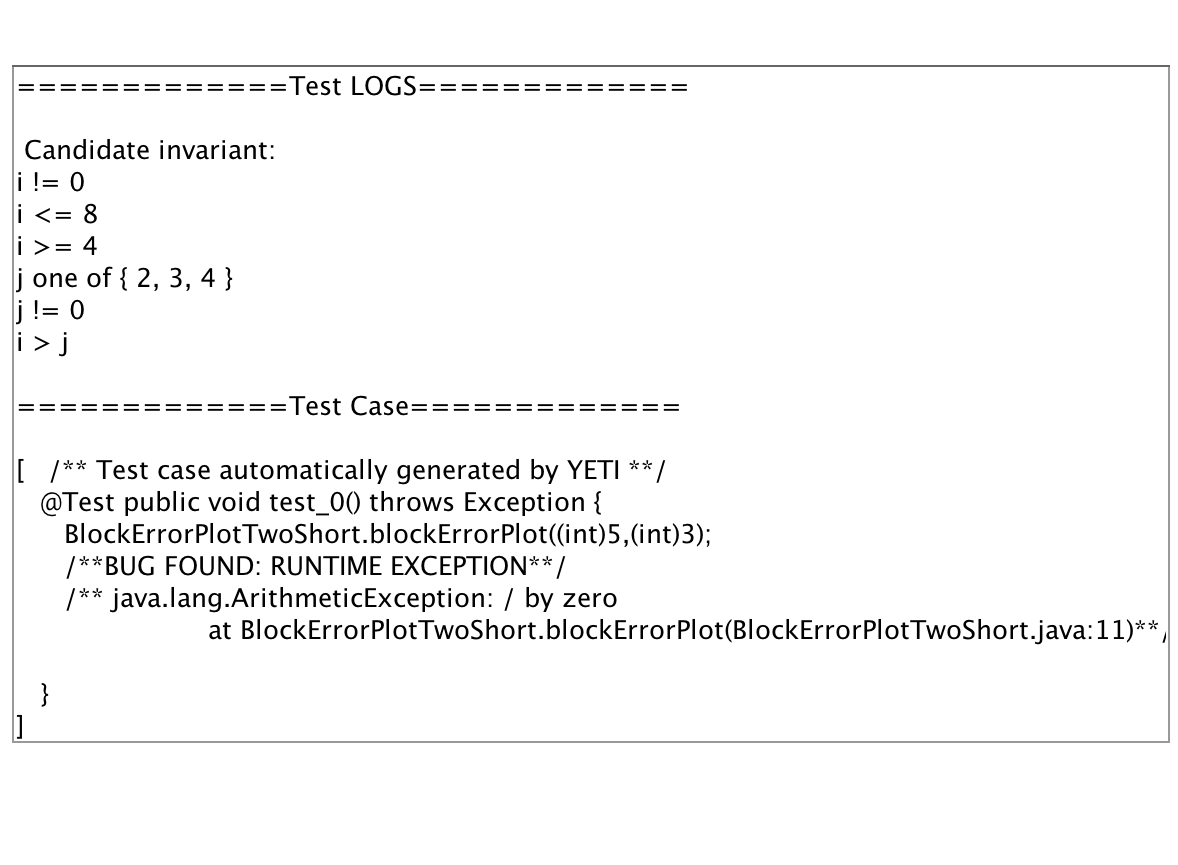
\includegraphics[width= 8.5cm,height=7cm]{adfdPlus2.png}
%\bigskip
%\caption{GUI front end of upgraded ADFD and ADFD$^+$}
%\label{fig:adfdUpgraded}
%\end{figure}





%Four of the above enhancements are visible from the front-end. As shown in Figure~\ref{fig:adfdUpgraded}, the drop down menu for strategy field enables the tester to choose the appropriate strategy in the list for the test session. Secondly, the block failure domain is shown in graphical form and with the help of automatic tool Daikon the failure domain is also shown  by invariants ( i one of \{-1, 0, 1\}, j == 0). Thirdly, the addition of YETI generated test case shows type of failure (RUNTIME EXCEPTION, java.lang.ArithmaticException: / by zero), name of the failing class (OneDimensionalBlockFailureDomain), name of the failing method (blockErrors), value causing the failure (1) and line number of the code causing failure (11). Fourthly, the provision of screen capture button allows the tester to store the record of each test for record.



%       ORIGINAL       %


%Prior to conducting the experiments for comparative evaluation, the ADFD and ADFD+ techniques were enhanced to increase the code coverage, provide information about the identified failure and generate invariants of the detected failure-domains as stated below.
%\begin{enumerate}

%\item Code coverage was increased by extending the techniques to support the testing of methods with byte, short, long, double and float arguments while it was restricted to int type arguments only in the original techniques.

%\item Additional information was facilitated by adding the YETI generated test case to the GUI of the two techniques. Test case includes the name of the failing method, values that caused the failure and stack trace of the failure.

%\item Invariants of the detected failure-domains were automatically generated by integrating the tool Daikon in the two techniques. Daikon is an automated invariant detector that detects likely invariants in the program~\cite{ernst2007daikon}. The generated invariants are displayed in the GUI of the techniques after completion of the test. 

%\end{enumerate}

\section{Difference in working mechanism of the two techniques}
Difference in working mechanism of ADFD and ADFD$^+$ for identification of failure domains is illustrated by testing a simple Java program (given below) with the two techniques. It is evident from the program code that failure is generated when the value of variable \textit{x = \{4, 5, 6, 7 or 8\}} and the corresponding value of variable \textit{y = \{2, 3 or 4\}}. The total number of 12 failing instances form a block failure domain in the input domain.

\begin{lstlisting}
/** 
* A program with block failure domain.
* @author (Mian and Manuel)
*/
public class BlockErrorPlotTwoShort {
	public static void blockErrorPlot (int x, int y) {
		if ((x >= 4) && (x <= 8) && (y == 2)) { 
			abort();		/* error */
		}
		if ((x >= 5) && (x <= 8) && (y == 3)) { 
			abort();		/* error */
		}
		if ((x >= 6) && (x <= 8) && (y == 4)) { 
			abort();		/* error */
		}
	}
}
\end{lstlisting}

The test output generated by ADFD technique is presented in Figure~\ref{fig:ADFD}. The labelled graph shows 4 out of 12 failing values in red whereas the passing values are shown in blue. The generated invariants identify all but one failing value ($x = 4$). This is due to the fact that ADFD scans the values in one-dimension around the failure. The test case shows the type of failure, name of the failing class, name of the failing method, values causing the failure and line number of the code causing failure.

\begin{figure}[h]
 \makebox[\textwidth][c]{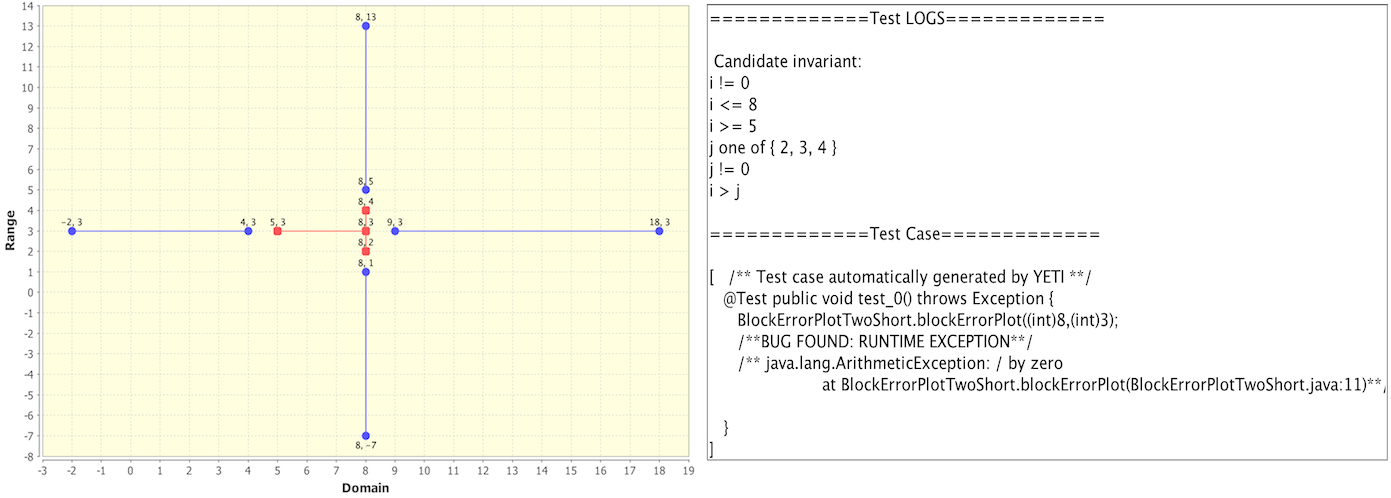
\includegraphics[width=1.2\textwidth]{adfdCombined.png}}%
%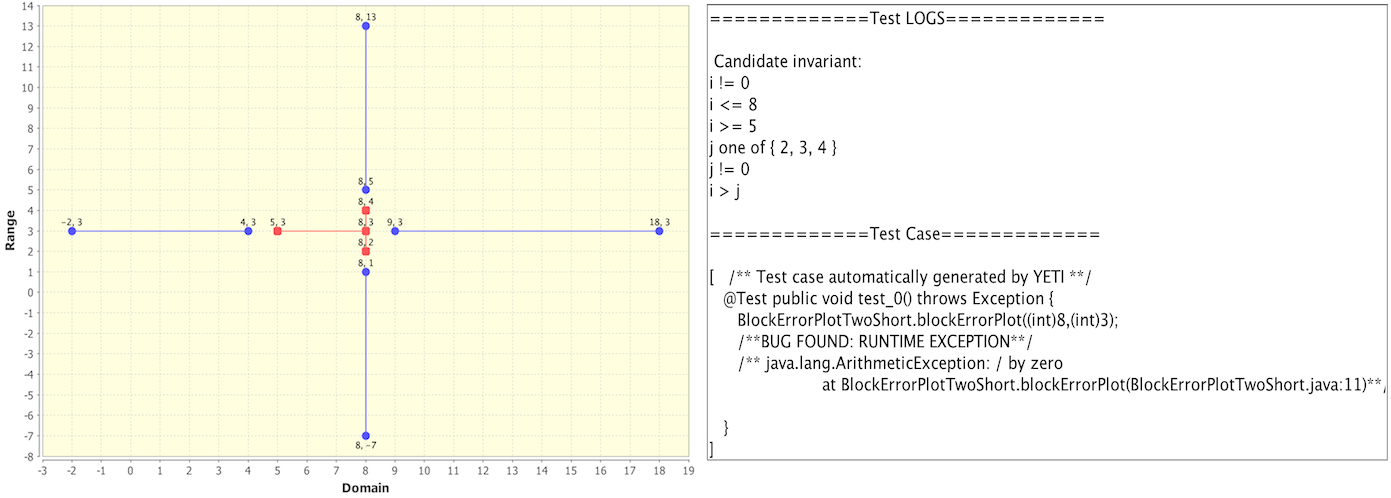
\includegraphics[width= 15cm,height=7cm]{adfdCombined.png}
\caption{Graph, Invariants and test case generated by ADFD for the given code}
\label{fig:ADFD}
\end{figure}

The test output generated by ADFD$^+$ technique is presented in Figure~\ref{fig:ADFD+}. The labelled graph correctly shows all the 12 out of 12 available failing values in red whereas the passing values are shown in blue. The invariants correctly represent the failure domain. The test case shows the type of failure, name of the failing class, name of the failing method, values causing the failure and line number of the code causing failure.

\begin{figure}[h]
\makebox[\textwidth][c]{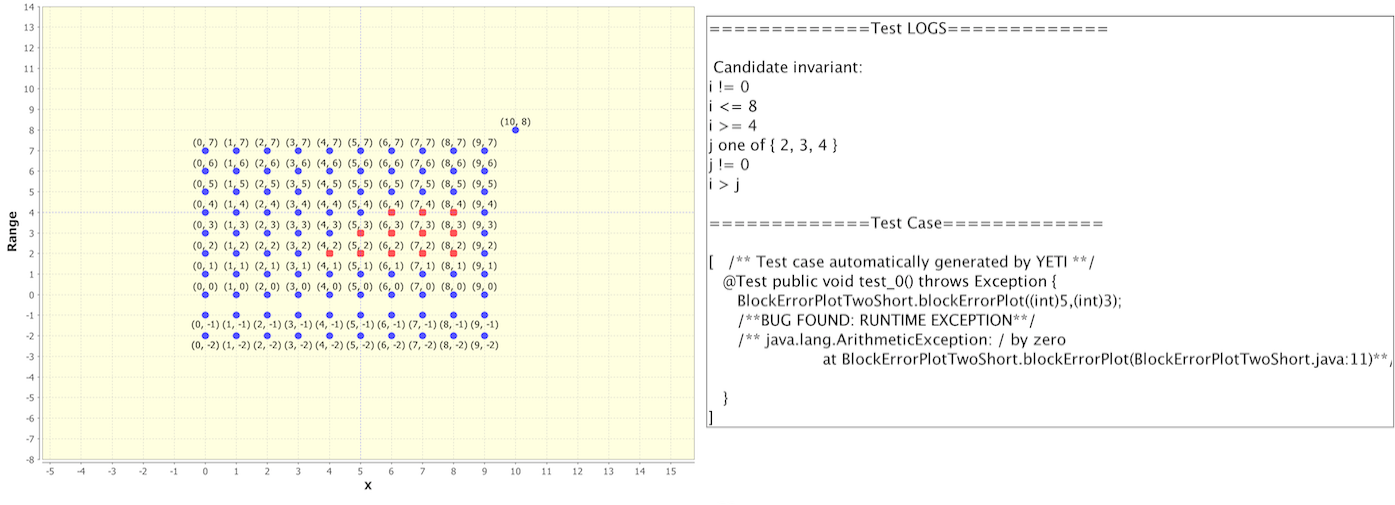
\includegraphics[width=1.2\textwidth]{adfdPlusCombined.png}}%
%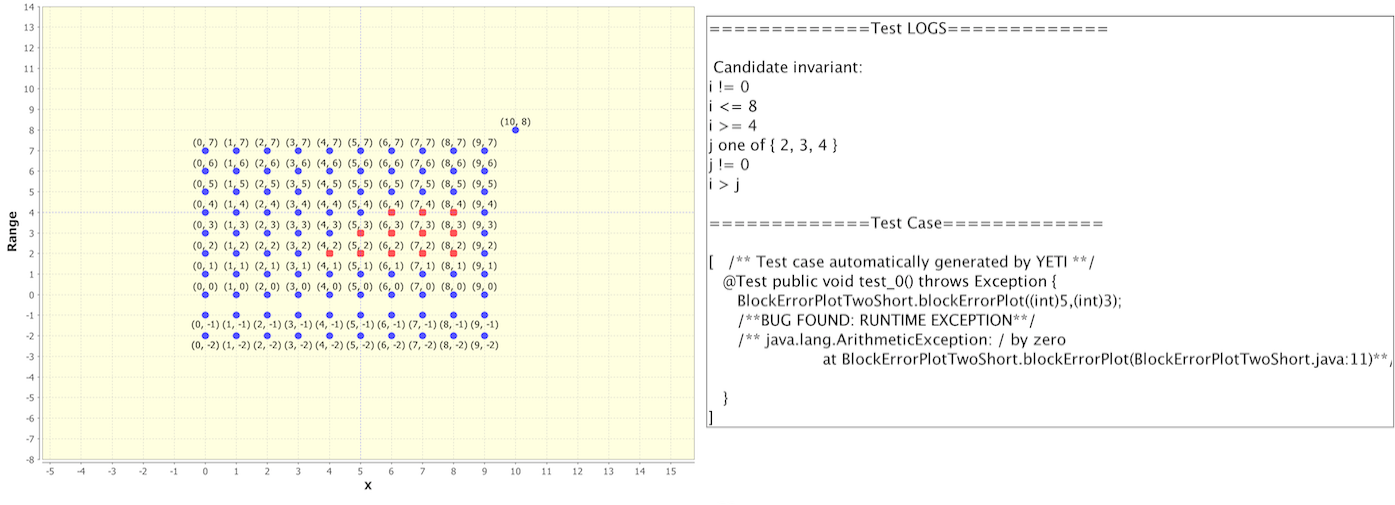
\includegraphics[width= 15cm,height=7cm]{adfdPlusCombined.png}
\caption{Graph, Invariants and Test case generated by ADFD$^+$ for the given code}
\label{fig:ADFD+}
\end{figure}


The comparative results derived from execution of the two techniques on the developed program indicate that, ADFD$^+$ is more efficient than ADFD in identification of failures in two-dimensional programs. The ADFD and ADFD$^+$ performs equally well in one-dimensional program, but ADFD covers more range around the first failure than ADFD$^+$ and is comparatively economical because it uses fewer resources than ADFD$^+$.




%      ORIGINAL     %

%The difference with respect to the identification of failure-domains is illustrated by testing a simple Java program (given below) with ADFD and ADFD+ techniques. 
%\smallskip
%\begin{lstlisting}
%/** 
%* A program with block failure-domain.
%* @author (Mian and Manuel)
%*/
%public class BlockErrorPlotTwoShort {
%	public static void blockErrorPlot (int x, int y){
%		int z;
%		if ((x >= 4) && (x <= 8) && (y == 2))
%			{ z = 50/0;}
%		if ((x >= 5) && (x <= 8) && (y == 3))
%			{ z = 50/0;}
%		if ((x >= 6) && (x <= 8) && (y == 4))
%			{ z = 50/0;}
%	}
%}
%\end{lstlisting}
%\smallskip
%As evident from the program code that an $ArithmeticException$ failure (divison by zero) is generated when the value of variable \verb+x one of {4, 5, 6, 7, 8}+ and the corresponding value of variable \verb+y one of {2, 3, 4}+. The values form a block failure-domain in the input domain. 

%\begin{figure}[H]
%\centering
%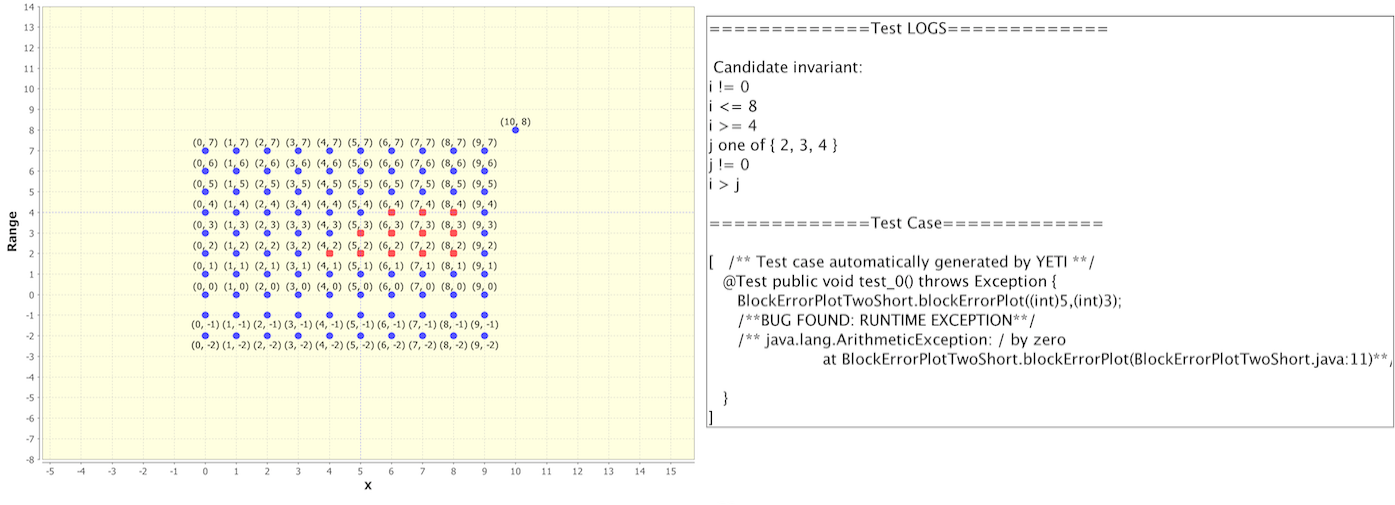
\includegraphics[width= 12.5cm,height=5.5cm]{adfdPlusCombined.png}
%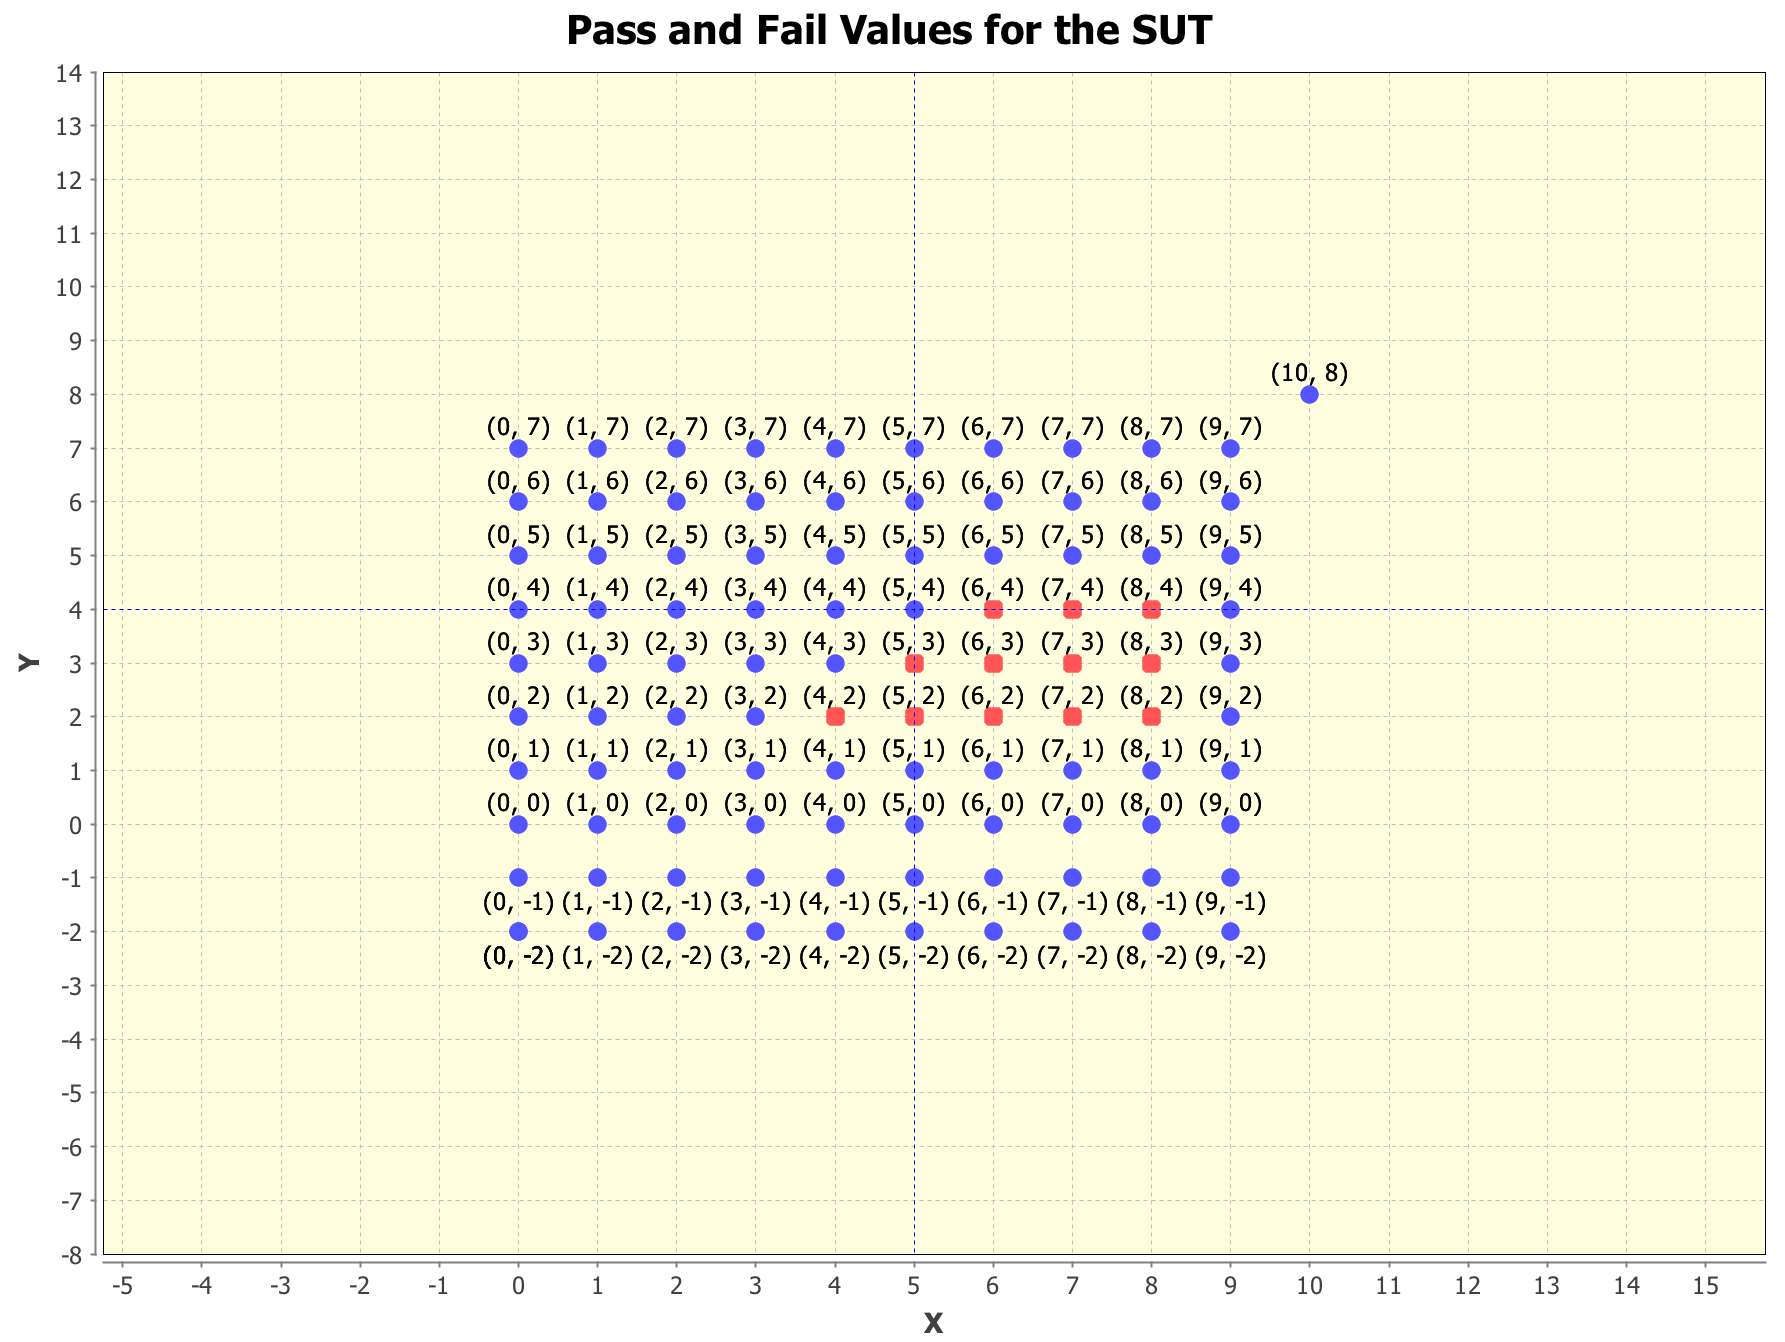
\includegraphics[width= 8.5cm,height=7cm]{adfdPlus1.png}
%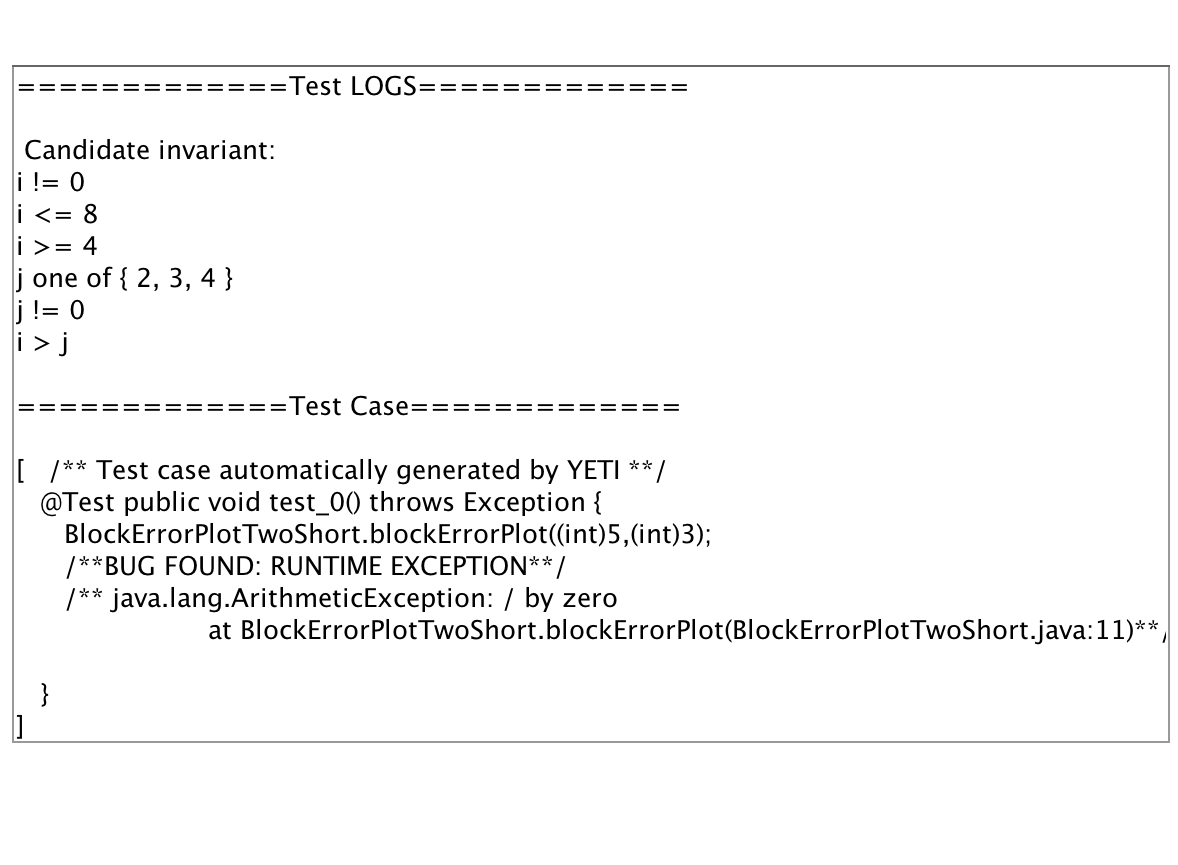
\includegraphics[width= 8.5cm,height=7cm]{adfdPlus2.png}
%\caption{Graph, Invariants and Test case generated by ADFD+}
%\label{fig:ADFD+}
%\end{figure}


%The test output generated by ADFD+ technique is presented in Figure~\ref{fig:ADFD+}. The labelled graph correctly shows all the 12/12 available failing values in red whereas the passing values are shown in blue. The invariants correctly represent the failure-domain. The test case shows the type of failure, the values causing the first failure and the stack trace of the failure.

%\begin{figure}[H]
%\centering
%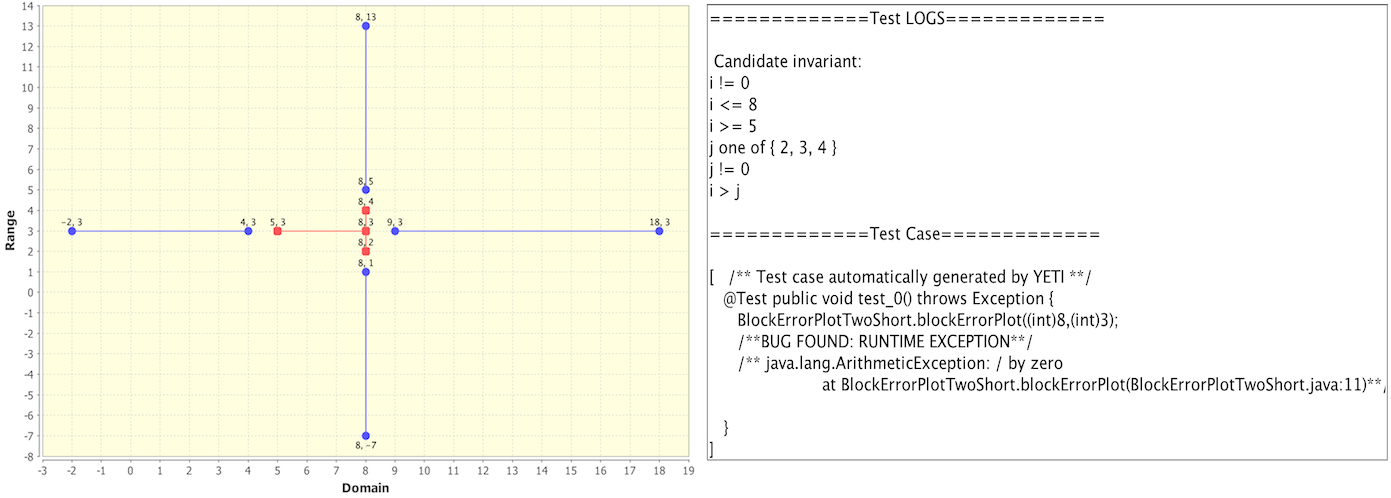
\includegraphics[width= 12.5cm,height=5.5cm]{adfdCombined.png}
%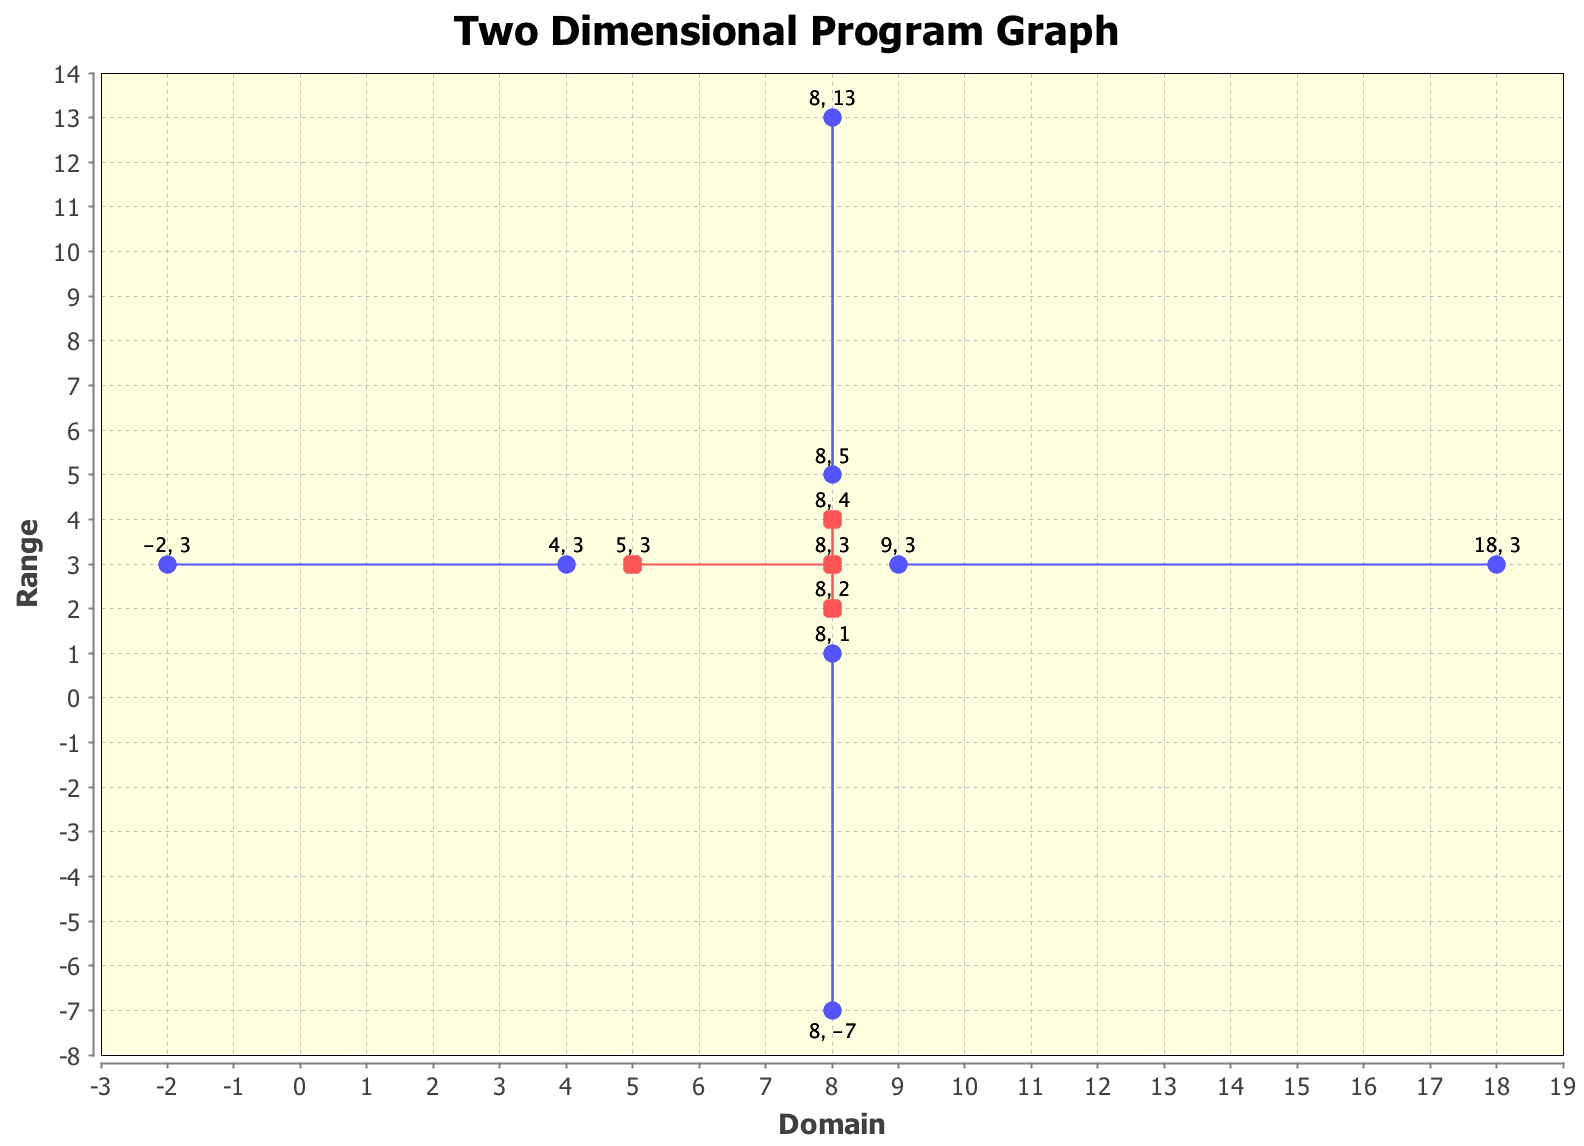
\includegraphics[width= 8.5cm,height=7cm]{adfdAround1.png}
%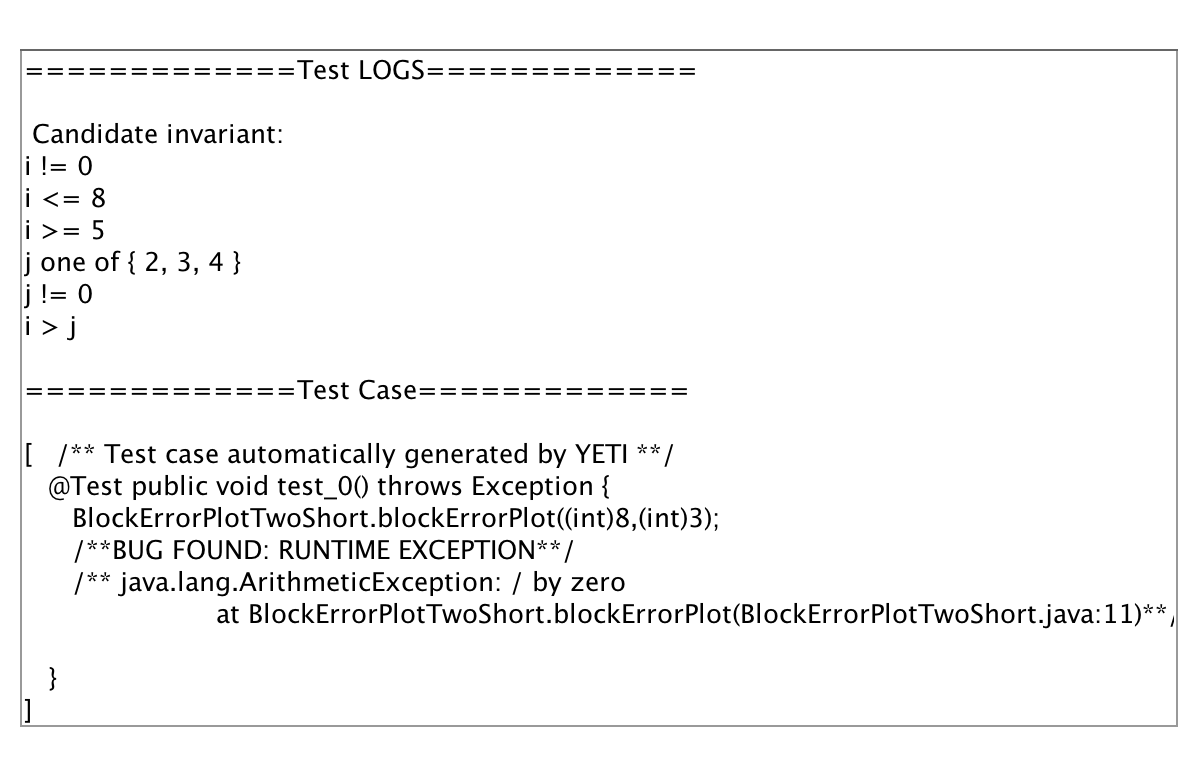
\includegraphics[width= 8.5cm,height=7cm]{adfdAround2.png}
%\caption{Graph, Invariants and test case generated by ADFD}
%\label{fig:ADFD}
%\end{figure}

%The test output generated by ADFD technique is presented in Figure~\ref{fig:ADFD}. The labelled graph correctly shows the 4/12 available failing values in red whereas the passing values are shown in blue. The invariants identify all but one failing values ($x = 4$). This is due to the fact that ADFD scans the values in one dimension around the failure. The test case shows the type of failure, the values causing the first failure and the stack trace of the failure. 

%The comparative results derived from the execution of the two techniques on the selected program indicate that ADFD+ is more efficient than ADFD in identification of failures in two dimensional program. ADFD and ADFD+ performs equally well in one-dimensional program but ADFD covers more range around the first failure than ADFD+ and is comparatively economical because it uses less resources than ADFD+.


\section{Research questions} \label{sec:questions}
The following research questions have been addressed in the study:
\begin{enumerate}
%

\item What is the relevance of ADFD and ADFD$^+$ techniques in identification and presentation of failure domains in production software?



% ORIGINAL %
%\item Can ADFD and ADFD+ techniques identify and present failure-domains in production software? %\\%The experimental results claiming the correct identification of ADFD and ADFD+ were based on the purpose build error-seeded programs~\cite{}. To answer the question, we applied the two techniques to all the projects of Qualitas Corpus and examined the results.

%\item \textit{If the graph and invariants generated, correctly represent the failure domains?} %Invariants generated by Daikon can identify the start and stop of the failure domain. To answer this question we compared the generated invariants with the source code and the failure-domain presented in graphical form.
%
%
\item What types and frequencies of failure domains exist in production software?
%\item What types and frequencies of failure-domains exist in production software? %\\%There are strategies~\cite{}.  that exploit the presence of block and strip failure-domain to get better results. Therefore identifying the presence of underlying failure-domains in production software can help in high quality of software testing.  To answer the questions, we reviewed all the classes containing failure-domains manually, automatically and graphically.
%
\item What is the nature of identified failure domain and how it affects the automated testing techniques?
%\item What is the nature of identified failure-domain and how it affects the testing techniques? % \\% An interesting point is to know what failure is responsible for a failure-domain and how difficult it is to identify that failure by manual testing. To answer this question, we studied the test logs and test output of the automated testing and the source code of the program manually to identify the cause and complexity of failures of failure-domains. 

%\item \textit{If the presence of a particular failure-domain can make it easy or hard to find using automated and manual techniques?} 
%Failure-domain can reside in the form of point, block or strip shape in the input domain. To answer this question we analysed the source code of all the programs in which failure-domains were detected.
%

%\item \textit{If the graph generated by ADFD correctly represent the pass and fail domains?} Both the ADFD and ADFD+ techniques generate graphs to represent failure-domains for simplicity. To answer the question we compared the generated graphs with the source code and the invariants generated by Daikon.
%
%\item If obtained results consistent with previous theoretical and practical results presented?  %As per our knowledge, till now no specific study has been conducted to automatically identify the pass and fail domains however it has been claimed by some researchers~\cite{} that there exist more block and strip patterns then the point patterns. 
%

%\item What is the external validity of the results obtained?\\

\end{enumerate}





\section{Evaluation}
Experimental evaluation of ADFD and ADFD$^+$ techniques was carried out to determine: the effectiveness of the techniques in identifying and presenting the failure domains, the types and frequencies of failure domains, the nature of error causing a failure domain and the external validity of the results obtained. 

%\section{Evaluation}
%Experimental evaluation of ADFD and ADFD+ techniques was carried out to determine: the effectiveness of the techniques in identifying and presenting the failure-domains, the types and frequencies of failure-domains, the nature of error causing failure-domain and the external validity of the results obtained. 

\subsection{Experiments}
In the present experiments, we tested all 106 packages of Qualitas Corpus containing the total of 4000 classes. Qualitas Corpus was selected because it is a database of Java programs that span across the whole set of Java applications and is specially built for empirical research which takes into account a large number of developmental models and programming styles. All packages included in Qualitas Corpus are open source with an easy access to the source code.

For experimental purpose, the main ``.jar'' file of each package was extracted to get the ``.class'' files as appropriate input for YETI. All 4000 classes were individually tested. The classes containing one and two-dimensional methods with arguments (int, long, float, byte, double and short) were selected for experimental analysis. Non-numerical arguments and more than two-dimensional methods were ignored because the two proposed techniques support the testing of one and two dimensional methods with numerical arguments. Each test took 40 seconds on the average to complete the execution. The initial 5 seconds were used by YETI to find the first failure while the remaining 35 seconds were jointly consumed by ADFD/ADFD$^+$ technique, JFreeChart and Daikon to identify, draw graph and generate invariants of the failure domains respectively. The machine took approximately 500 hours to perform the experiments completely. Due to the absence of contracts and assertions in the code under test, undeclared exceptions were taken as failures in accordance with the previous studies~\cite{oriol2012random}, \cite{ahmad2013adfd}. The source code of the programs containing failure domains were also evaluated manually to cross-examine the experimental results. 

In accordance with Chan et al.~\cite{chan1996proportional}, classification of failure domain into various types was based on the number of contiguous failures detected in the input-domain as shown in Table~\ref{table:resultsSummary}. If the contiguous failures detected range from 1 to 5, 6 to 49 or 50 and above the failure domain is classified as point, block or strip type respectively. If more than one type of domain are detected in a program, it is termed as mix type. 

\begin{table}[h]
\scriptsize
\caption{Classification of failure domains} 
\centering
{\renewcommand{\arraystretch}{1.5}
\begin{tabular}{| r | l | l |} 
\hline 
S. No 	&	Type of failure domain						& No of contiguous failures	 \\
				  
				 
				 
				 
\hline 
1		&	Point										 & 01 to 05							\\
\hline 
2		& 	Block										 & 06 to 49							\\
\hline 
3		&	Strip 										 & 50 \& above						 \\ 
%Mix													 &									\\
\hline 
		&				 								 & point \& block						\\
4		& 	Mix											 & point \& strip 						\\
		&											        & point, block \& strip				\\
\hline
\end{tabular}
}
\label{table:resultsSummary} % is used to refer this table in the text
\end{table}

%All experiments were conducted with a 64-bit Mac OS X Mountain lion version 10.8.5 running on 2.7 GHz Intel Core i7 with 16 GB (1600 MHz DDR3) of RAM. YETI runs on top of the Java\texttrademark  SE Runtime Environment [version 1.7.0\_45]. The ADFD and ADFD$^+$ executable files are available at \url{https://code.google.com/p/yeti-test/downloads/list/}. Daikon and JFreeChart can be seperately obtained from \url{http://plse.cs.washington.edu/daikon/} and \url{http://www.jfree.org/jfreechart/download.html} respectively. 




%\subsection{Experiments}
%In the present experiments we tested all 106 packages of Qualitas Corpus containing the total of 4000 classes. Qualitas Corpus was selected because it is a database of Java programs that spans across the whole set of Java applications, it is specially built for empirical research which takes into account a large number of developmental models and programming styles. Its all included packages are open source with an easy access to the source code.




%Since YETI tests the byte code only therefore the main ``.jar'' file of each package was extracted to get the ``.class'' files. Each class was individually tested. The one and two dimensional methods with arguments (int, long, float, byte, double and short) of each class were selected for experimental testing. Non numerical arguments and more than two dimensional methods were ignored because the two proposed techniques support the one and two dimensional methods with numerical arguments. Each test took 40 seconds on the average to complete the execution. The initial 5 seconds were used by YETI to find the first failure while the remaining 35 seconds were jointly consumed by ADFD/ADFD+ technique, JFreeChart and Daikon to identify, draw graph and generate invariants of the failure-domains respectively. The machine took approximately 100 hours to perform the experiments. Due to the absence of contracts and assertions in the code under test, undeclared exceptions were taken as failures in accordance with the previous studies~\cite{ahmad2013adfd}\cite{oriol2012random}. The source code of the programs containing failure-domains were also evaluated manually to cross-examine the experimental results. All experiments were conducted with a 64-bit Mac OS X Mountain lion version 10.8.5 running on 2.7 GHz Intel Core i7 with 16 GB (1600 MHz DDR3) of RAM. YETI runs on top of the Java\texttrademark  SE Runtime Environment [version 1.7.0\_45]. The ADFD and ADFD+ executable files are available at \url{https://code.google.com/p/yeti-test/downloads/list/}. 



\subsection{Results}
The testing of 106 Java packages including 4000 classes, resulted in 25 packages containing 57 classes to have various types of failure domains. The details pertaining to project, class, method, dimension, line of code (LOC) and type of detected failure domains for each class are given in Table 3. Out of the total of 57 methods indicated in the table, 10 methods are two-dimensional while the remaining 47 methods are one-dimensional. A total number of 17262 lines of code spread across 57 classes in various proportions as shown in the table. The results obtained show that out of 57 classes 2 contain point failure domain, 1 contains block failure domain, 50 contain strip failure domain and 4 contain mix failure domain. %Mix failure domain includes the combination of two or more types of failure domains including point \& block, point \& strip and point, block \& strip. 



%Among 106 packages we found 25 packages containing 57 classes with different types of failure-domains. Based on the type of failure-domains the results are presented in Table \ref{table:stripDomains}, \ref{table:pointDomains}, \ref{table:blockDomains}, \ref{table:mixDomains}. The information available in the table includes the class showing failure domain, the method involved, the invariants generated by ADFD and ADFD+ (automatic techniques) and by manual analysis. 

%Classification of failure-domains into strip, point, block and mix types is based on the degree of contiguity of failures detected in the input-domain as shown in Table~\ref{table:results}. If failures detected as contiguous are 50 or more, the failure-domain is classified as strip.  If failures detected as contiguous lie in the range of 1 to 5, the failure domain is classified as point. If failures detected as contiguous lie in the range of 6 to 49, the failure domain is classified as block. If more than one type of failure domains are detected in the input domain, the domain is classified as mix.

%The results obtained show that out of 57 classes 50 contain strip failure domain,2 contain point failure domain, 1 contain block failure domain and 4 contain mix failure domain. Mix failure-domain includes the combination of two or more failure domain types including point \& strip, point \& block and point, block \& strip. Invariants generated by manual and automated techniques, and analysis of the source code is also performed to differentiate the simplicity and complexity of the identified failure-domains as shown in Table~\ref{table:results}. Further explanation is available in the Nature of failure-domain subsection. The key research questions identified in the previous section are individually addressed in the following.


%The failure-domains were declared as strip failure-domains if 50 or more contagious failures were detected. 
%Accordingly, in 48 out of 57 classes strip failure-domains were detected as shown in Table~\ref{table:stripDomains}. 

%The failure-domains were declared as point failure-domains if more than 1 and less than 5 contagious failures were detected. Accordingly, in 4 out of 57 classes point failure-domains were detected as shown in Table~\ref{table:pointDomains}.

%The failure-domains were declared as block failure-domains if more than 5 and less than 50 contagious failures were detected. Accordingly, in 2 out of 57 classes block failure-domains were detected as shown in Table~\ref{table:blockDomains}.

%The remaining 2 classes contained two types of failure-domains i.e one containing both point and block failure-domain and the other containing point and Strip failure-domain as shown in Table~\ref{table:mixDomains}.


%\begin{table}[h]
%\scriptsize
%\caption{Results of the experiments} 

%\centering
%{\renewcommand{\arraystretch}{1.5}
%\begin{tabular}{| l | l | l | l | l | l | l | l | l | l | l | } 
%\hline 
%Failure domain	& Contiguous failures	 & \rot{90}{No. of classes} 	& \rot{90}{No. of failure-domains}   & \rot{90}{Easy to Find FD by ADFD} & \rot{90}{Easy to Find FD by ADFD+}	& \rot{90}{Easy to Find FD by MT} & \rot{90}{Hard to find FD by ADFD} & \rot{90}{Hard to find FD by ADFD+} & \rot{90}{Hard to find FD by ADFD+}\\
				 
				 
				 
				 
%\hline 
%Strip 			 & 50 or more				&	50			&	50		& 50 	& 45 	& 48 	& 0 		& 5 		& 2 \\ 
%Point			 & between 1 and 5			&	2			&	2		& 2   	& 2		& 2		& 0 		& 0 		& 0 \\
%Block			 & between 6 and 49			&	1			&	1		& 0		& 1		& 1		& 1		& 0		& 0\\
%Mix				 &							&				&			& 		& 		& 		& 		&		&  \\
%				 & point and strip 			& 	3			&	3		& 3		& %0		& 2		& 0		& 3		& 1\\
%				 & point and block			&	0			&	0   		& 0		& 0		& 0		& 0		& 0		& 0\\
%				 & point, block \& strip		&     1 			&	1		& 1		& 0 		& 0 		& 0		& 1		& 1\\
%\hline
%Total			 & 							&    57  			&	57		& 57	& 48 	& 53	& 1		& 9		& 4\\
%\hline
%\end{tabular}
%}
%\label{table:results} % is used to refer this table in the text
%\end{table}




\subsubsection{Effectiveness of ADFD and ADFD$^+$ techniques}
The experimental results confirmed the effectiveness of the techniques by discovering all three types of failure domains (point, block and strip) across the input domain. The results obtained by applying the two automated techniques were verified: by manual analysis of the source code of all 57 classes; by cross checking the test case, the graph and the generated invariants of each class; by comparing the invariants generated by automatic and manual techniques. 

The identification of failure domain by both ADFD and ADFD$^+$ is dependant upon the detection of failure by random$^+$ strategy in YETI. Because only after a failure is identified, its neighbouring values are analysed according to the set range to plot the failure domain.

The generation of graph and invariants and the time of test execution directly depends on the range value, if the range value of a technique is greater, the presentation of failure domain is better and the execution time required is higher. This is due to the testing and handling of greater number of test cases when the range is set to a bigger level. Comparatively, ADFD requires fewer resources than ADFD$^+$ therefore it is less influenced by the range value.

%\subsubsection{Effectiveness of ADFD and ADFD+ techniques:}
%The effectiveness of ADFD and ADFD+ techniques for identifying failure-domains in production software was demonstrated. The experimental results confirmed the effectiveness of the techniques by discovering all three types of failure-domains (point, block and strip) across the input domain. The results obtained by applying the two automated techniques were verified: by manual analysis of the source code of all 57 classes containing failure domains; by cross checking the test case, the graph and the generated invariants of each class; by comparing the invariants generated by automatic and manual techniques. 

%The identification of failure domain by both ADFD and ADFD+ is dependant on the identification of failure by ADFD and ADFD+ strategy in YETI. Because only after a failure is identified, its neighbour values according to the set range are analysed and failure domain of the failure is plotted.

%The generation of graph and invariants depends on range value, the greater the range value of a technique the better is the presentation of failure domain. The generation of graph and invariants starts from the minimum range value and ends at the maximum range value around the detected failure value. The ADFD requires less resources and is thus capable of handling  greater range value as compared to ADFD+.  




%For example consider the following code under test. If the range value of ADFD is from -100 to 100 and the range value for ADFD+ is from -10 to 10 then the invariants generated to represent the failure domain by ADFD will be $ i one of \{ -1, -100 \} $ while for ADFD+ they will be $ i one of \{-1, -10\} $. Similarly the invariants generated to represent the failure-domain manually will be $ i <= -1 $. The presentation can be further improved if the value of range is extended to Integer.MIN\_INT and Integer.MAX\_INT . 

%\smallskip
%\begin{lstlisting}
%/** 
%* A program with strip failure-domain.
%* @author (Mian and Manuel)
%*/
%public class StripErrorPlot {
%	public static void stripErrorPlot (int x){
%		int a[] = new int[x];
%	}
%}
%\end{lstlisting}
%\smallskip 

%With all the effectiveness of automated techniques we still believe that ADFD and ADFD+ cannot be used as replacement of manual testing however it should be used to assist the manual testing for achieving higher quality.


\subsubsection{Type and Frequency of Failure domains}

As evident from the results given in Table 4 - 7, all the three techniques (ADFD, ADFD$^+$ and Manual) detected the presence of strip, point and block types of failure domains in different frequencies. The results obtained show that out of 57 classes 2 contain point failure domain, 1 contains block failure domain, 50 contain strip failure domain and 4 contain mix failure domain. Mix failure domain includes the combination of two or more types of failure domains including point \& block, point \& strip and point, block \& strip.

%Out of 57 classes containing failure domains, 50 classes showed strip failure domain, 2 point failure domain, 1 block failure domain and 4 mix failure domains.  

The discovery of higher number of strip failure domains may be attributed to the fact that a limited time of 5 seconds were set in YETI testing tool for searching the first failure. The ADFD and ADFD$^+$ strategies set in YETI for testing the classes are based on random$^+$ strategy which gives high priority to boundary values, therefore, the search by YETI was prioritised to the boundary area where there were greater chances of occurrence of failures constituting strip failure domain.

%It may be noted that YETI, which is used to find the first failure, is executed only for five seconds which uses ADFD and ADFD+ testing strategies. Both the strategies are based on random+ strategy which gives high priority to boundary values. It may be possible that the high number of strip failure-domains are detected because most of the failures are found at the boundaries.


%\subsubsection{Type and Frequency of Failure-domains:}
%As evident from the results given in Table 3 - 6, all the three techniques (ADFD, ADFD+ and Manual) detected the presence of strip, point and block types of failure domains in different frequencies. Out of 57 classes containing failure domains, 50 classes showed strip failure domain, 2 point failure domain, 1 block failure domain and 4 mix failure domains.  

%The discovery of higher number of strip type of failure domains may be attributed to the fact that a limited time of 5 seconds were set in YETI testing tool for searching the first failure. The ADFD and ADFD+ strategies set in YETI for testing the classes are based on random+ strategy which gives high priority to boundary values, therefore the search by YETI was prioritised to the boundary area where there were greater chances of occurrence of failures constituting strip type of failure domain.

%It may be noted that YETI, which is used to find the first failure, is executed only for five seconds which uses ADFD and ADFD+ testing strategies. Both the strategies are based on random+ strategy which gives high priority to boundary values. It may be possible that the high number of strip failure-domains are detected because most of the failures are found at the boundaries.

% ADD TABLES AT THE END RELATED TO THIS SECTION %


\subsubsection{Nature of failure domain} \label{sec:nature}
The nature of failure domain identified by two automatic techniques (ADFD and ADFD$^+$) and the manual technique was examined in terms of simplicity and complexity by comparing the invariants generated by automatic techniques with those of the manual technique. The results were split into six categories (2 categories per technique) on the basis of simplicity and complexity of failure domains identified by each of the three techniques. The comparative results show that ADFD, ADFD$^+$ and Manual testing can easily detect 56, 48 and 53 and difficultly detect 1, 9 and 4 failure domains respectively as shown in Table~\ref{table:simpleComplex}. The analysis of generated invariants indicate that the failure domains which are simple in nature are easily detectable by both automated and manual techniques while the failure domains which are complex in nature are difficultly detectable by both automated and manual techniques. %Both types are explained with the help of following examples.

\begin{table}[h]
\scriptsize
\caption{Simplicity and complexity of Failure Domains (FD) as found by 03 techniques} 
\centering
{\renewcommand{\arraystretch}{1.5}
\begin{tabular}{| c | r | r | r | r | r | r | r | r | } 
\hline 
\rot{90}{\pbox{20cm}{Type of \\failure domain}}	& \rot{90}{\pbox{20cm}{No. of \\classes}} 	& \rot{90}{\pbox{20cm}{No. of \\FD}}   & \rot{90}{\pbox{20cm}{Easy to find \\FD by ADFD}} & \rot{90}{\pbox{20cm}{Easy to find \\FD by ADFD$^+$}}	& \rot{90}{\pbox{20cm}{Easy to find \\FD by MT}} & \rot{90}{\pbox{20cm}{Hard to find \\FD by ADFD}} & \rot{90}{\pbox{20cm}{Hard to find \\FD by ADFD$^+$}} & \rot{90}{\pbox{20cm}{Hard to find \\FD by MT}}\\

%\rot{90}{failure domain}	& \rot{90}{No. of classes} 	& \rot{90}{No. of FD}   & \rot{90}{Easy to find FD by ADFD} & \rot{90}{Easy to find FD by ADFD$^+$}	& \rot{90}{Easy to find FD by MT} & \rot{90}{Hard to find FD by ADFD} & \rot{90}{Hard to find FD by ADFD$^+$} & \rot{90}{Hard to find FD by MT}\\
				 
				 
				 
\hline 
Point			 &	2			&	2		& 2   	& 2		& 2		& 0 		& 0 		& 0 \\
\hline 
Block			 &	1			&	1		& 0		& 1		& 1		& 1		& 0		& 0\\
\hline 
Strip 			 &	50			&	50		& 50 	& 45 	& 48 	& 0 		& 5 		& 2 \\ 
%Mix			 &				&			& 		& 		& 		& 		&		&  \\
\hline 
				 &	0			&	0   		& 0		& 0		& 0		& 0		& 0		& 0\\
Mix				 & 	3			&	3		& 3		& 0		& 2		& 0		& 3		& 1\\
				 &   1 			&	1		& 1		& 0 		& 0 		& 0		& 1		& 1\\
\hline
Total			 &   57  			&	57		& 57	& 48 	& 53	& 1		& 9		& 4\\
\hline
\end{tabular}
}
\label{table:simpleComplex} % is used to refer this table in the text
\end{table}



The simplicity of failure domain is illustrated by taking an example of ADFD, ADFD$^+$ and Manual Analysis in Table 7 for class BitSet. The negativeArray failure is detected due to the input of negative value to the method bitSet.of(i). The invariants generated by ADFD are \textit{\{i $\le$ -1, i $\ge$ -18\}}, by ADFD$^+$ are \textit{\{i $\le$ -1, i $\ge$ -512\}} and by Manual Analysis are \textit{\{i $\le$ -1, i $\ge$ Integer.MIN\_INT\}}. These results indicate maximum degree of representation of failure domain by Manual Analysis followed by ADFD and ADFD$^+$ respectively. This is mainly due to the bigger range value in manual analysis followed by ADFD and ADFD$^+$ respectively. 


%It was also found that ADFD+ is capable of identifying the failure domain to the large degree of accuracy in the case of point and block failure domain but not in the strip failure domain. While ADFD and Manual techniques are capable of correctly identifying all type of failure domain.

The complexity of failure domain is illustrated by taking an example of ADFD, ADFD$^+$ and Manual Analysis in Table 7 for class ArrayStack. The \verb+OutOfMemoryError+ failure is detected due to the input of value to the method ArrayStack(i). The invariants generated by ADFD are \textit{\{ i $\ge$ 698000000, i $\le$ 698000300\}}, by ADFD$^+$ are \textit{\{ i $\ge$ 2147483636, I $\le$ MAX\_INT\}}, by Manual analysis \textit{\{ i $\ge$ 698000000 \}}. All the three strategies indicate the same failure but at different intervals. The ADFD$^+$ is unable to show the starting point of failure due to its small range value. The ADFD easily discovers the breaking point due to its bigger range value while manual testing requires over 50 attempts to find the breaking point.




%\subsubsection{Nature of failure-domain:}
%The nature of failure domain as identified by automatic techniques (ADFD and ADFD+) and Manual technique was examined in terms of simplicity and complexity by comparing the invariants generated by the automatic techniques with the manual technique. The results were split into six categories on the basis of simplicity and complexity of failure-domains identified by each technique. The comparative results show that ADFD, ADFD+ and Manual testing can easily detect 56, 48 and 53 and difficultly detect 1, 9 and 4 failure domains respectively as shown in ~\ref{table:results}.

%The analysis of generated invariants indicated that the failure domains which are simple in nature are easily detectable by both automated and manual techniques irrespective of the type of failure domain (Strip, point, block). It was further indicated that the failure domains which are complex in nature are difficultly detectable by both automated and manual techniques. %Both types are explained with the help of following examples.
%Consider the following class with a simple failure domain detectable by all three techniques, we consider the results of ADFD, ADFD+ and Manual Analysis in Table 1 for class BitSet. The negativeArray failure is detected due to the input of negative value to the method bitSet.of(i). The invariants generated by ADFD are $\{i <= -1, i >= -18\}$, by ADFD+ are $\{i <= -1, i >= -512\}$ and by Manual Analysis are $\{i <= -1, i >= Integer.MIN\_INT\}$. These results indicate maximum degree of representation of failure-domain by Manual Analysis followed by ADFD and ADFD+ respectively.

%It was also found that ADFD+ is capable of identifying the failure domain to the large degree of accuracy in the case of point and block failure domain but not in the strip failure domain. While ADFD and Manual techniques are capable of correctly identifying all type of failure domain.

%As an example of complex failure, we consider the results of ADFD, ADFD+ and Manual Analysis in Table 1 for class ArrayStack. The OutOfMemoryError failure is detected due to the input of value to the method ArrayStack(i). The invariants generated by ADFD are $\{ i >= 2147483636, I <= 2147483647\}$, by ADFD+ are $\{ i >= 2147483142, i <= 2147483647\}$, by Manual analysis $\{ i >= 698000000 \}$.



%Easy to find were those in which negativearraysizeexceptin.
%hard to find were those like IndexArrayOutOfBoundsException.
%Impossible to find were those in which finding failure is easy but finding the cut over point is very difficult. like OutOfMemoryError.


%\subsubsection{External validity of Results:}
%The external validity is the degree to which the subject packages are representative of true practice. 





%\section{Experimental results} \label{sec:result}
%The experimental results show that the ADFD+ outperformed Randoop in both the time taken and number of tests used to detect all the injected faults. The ADFD+ also provide the added benefit of presenting the results in graphical form as shown in Figure \ref{fig:failureDomainsOneDimension} and \ref{fig:failureDomainsTwoDimension}. 
%Results are split in to two sections depicting efficiency and effectiveness of the two tools.
%\subsection{Efficiency}
%Figure \ref{fig:testtime} shows the comparative efficiency of ADFD+ and Randoop. The $x-axis$ represents one and two-dimensional programs with point, block and strip failure domains while the $y-axis$ represents average time taken by the tools to detect the failure domains. As shown in the figure ADFD+ showed extra ordinary efficiency by taking two orders of magnitude less time to discover failure domains as compared to Randoop. 

%This may be partially attributed to the very fast processing of YETI, integrated with ADFD+. YETI is capable of executing $10^6$ test calls per minute on Java code. To counter the contribution of YETI and assess the performance of ADFD+ by itself, the effectiveness of ADFD+ was compared with Randoop in terms of the number of test cases required to identify the failure domains without giving any consideration to the time consumed for completing the test session. The results are presented in the following section.

%It should be noted that the part of the gain may also be due to the fast processing of the underlying tool YETI, which is capable of executing $10^6$ test calls per minute on Java code. Therefore, to find the performance of only ADFD+ we performed the second set of experiments to measure effectiveness.

%For finding the efficiency, the CPU time consumed from the start of the test to the identification of last failure was measured for each experiment of ADFD+ and Randoop.  Figure \ref{fig:testtime} shows the results in a box-and-whisker plot. The figure shows that ADFD+ in no case took more than ten seconds to find the failures where Randoop consumed at least  80 seconds to find the same failures.
%\subsection{Effectiveness}
%Figure \ref{fig:testcases} shows the comparative effectiveness of ADFD+ and Randoop. The $x-axis$ represents one and two-dimensional programs with point, block and strip failure domains while the $y-axis$ represents average number of test cases used by the tools to detect the failure domains. The figure shows higher effectiveness in case of ADFD+, amounting to 100\% or more. The higher effectiveness of ADFD+ may be attributed to its working mechanism in comparison with Randoop for identifying failures. ADFD+ dynamically changes its algorithm to exhaustive testing in a specified radius around the failure as against Randoop which uses the same random algorithm for searching failures.

%\subsection{Failure Domains}
%The comparative results of the two tools with respect to presentation of the identified failure domains reveal better performance of ADFD+ by providing the benefit of presenting the failure domains in graphical form as shown in Figure \ref{fig:failureDomainsOneDimension} and \ref{fig:failureDomainsTwoDimension}. The user can also enable or disable the option of showing the failing values on the graph. In comparison Randoop lacks the ability of graphical presentation and the option of showing the failure domains separately and provides the results scattered across the textual files. 
 
 












%\section{Discussion}\label{sec:discussion}
%The results indicated that ADFD+ is a promising technique for finding failure and failure domain efficiently and effectively. It has the added advantage of showing the results in graphical form. The pictorial representation of failure domains facilitates the debuggers to easily identify the underlying failure domain and its boundaries for troubleshooting.


%In the initial set of experiments Randoop was executed for several minutes with default settings. The results indicated no identification of failures after several executions. On analysis of the generated unit tests and Randoop's manual, it was found that the pool of values stored in Randoop database for int primitive type contains only 5 values including -1, 0, 1, 10 and 100. To enable Randoop to select different values, we supplied a configuration file with the option to generate random values between -500 and 500 for the test cases as all the seeded errors were in this range. 

%As revealed in the results ADFD+ outperformed Randoop by taking two orders of magnitude less time to discover the failure domains. This was partially attributed to the very fast processing of YETI integrated with ADFD+. To counter the effect of YETI the comparative performance of ADFD+ and Randoop was determined in terms of the number of test cases required to identify the failure domains giving no consideration to the time taken for completing the test session. As shown in the results ADFD+ identified all failure domains in 50\% or less number of test cases.


%The ADFD+ was found quite efficient and effective in case of block and strip domains but not so in case of point domains where the failures lied away from each other as shown in the following code. This limitation of ADFD+ may be due to the search in vain for new failures in the neighbourhood of failures found requiring the additional test cases resulting in increased overhead.\\

%\begin{lstlisting}
%public class Error {
  %public static void Error (int x, int y){
  %	int z;
%	if (x == 10000)
%		 {	z = 50/0;	}
%		 
%	if (y == -2000)
%		 {	z = 50/0;	}
  % } 
%}
%\end{lstlisting}


%The number of test cases to be undertaken in search of failures around the previous failure found is set in the range value by the user. The time taken by test session is directly proportional to the range value.  Higher range value leads to larger graphical output requiring zoom feature which has been incorporated in ADFD+ for use when the need arise.



\section{Threats to validity} \label{sec:threat}
All packages in Qualitas Corpus were tested by ADFD, ADFD$^+$ and Manual technique in order to minimize the threats to external validity. The Qualitas Corpus contains packages of different: functionality, size, maturity and modification histories.

YETI using ADFD/ADFD$^+$ strategy was executed only for 5 seconds to find the first failure in the given SUT. Since both ADFD and ADFD$^+$ are based on random$^+$ strategy having high preference for boundary values, therefore, most of the failures detected are from the boundaries of the input domain. It is quite possible that increasing the test duration of YETI may lead to the discovery of new failures with different failure domain.

A threat to validity is related to the hardware and software resources. For example, the \verb+OutOfMemoryError+ occurs at the value of 6980000 on the machine used for executing the test. On another machine with different specification the failure revealing value can increase or decrease depending on the hardware and software resources.

It is to point out that all non-numerical and more than two-dimensional methods were not considered in the experiments. The failures caught due to error of non-primitive type were also ignored because of the inability of the techniques to present them graphically. Therefore, the results may reflect less number of failures.



%\section{Threats to validity} \label{sec:threat}
%All packages in Qualitas Corpus were tested by ADFD, ADFD+ and Manual techniques in order to minimize the threats to external validity. The Qualitas Corpus contains packages of different: functionality, size, maturity and modification histories.

%YETI using ADFD/ADFD+ strategy was executed only for 5 seconds to find the first failure in the given SUT. Since both ADFD and ADFD+ strategies are based on random+ strategy having high preference for boundary values therefore most of the failures detected are from the boundaries of input domain. It is quite possible that increasing the test duration of YETI may lead to the discovery of new failures with different failure domain.

%Another threat to validity is related to the hardware and software resources. For example the OutOfMemoryError occured at the value of 6980000 on the machine executing the test. On another machine with different specification the failure revealing value can increase or decrease depending on the hardware and software.

%It may be noted that all the non numerical and more than two dimensional methods were not considered in the experiments. The failures caught due to the error of non primitive type were also ignored because of the inability to present them. Therefore the results may reflect less number of failures.










%The study faces threats to external and internal validity. The external threats are common to most of the empirical evaluations. It includes the extent to which the programs under test the generation tools and the nature of seeded errors are representative of the true practice. The present findings will serve as foundation for future research studies needed to be undertaken with several types of classes, test generation tools and diversified nature of seeded errors in order to overcome the threats to external validity. The internal threats to validity includes error-seeded and limited number of classes used in the study. These may be avoided by taking real and higher number of classes in future studies.

\section{Related Work}
Shape and location of failure domain within the input domain have been studied in the past. Similar to our findings, White et al.~\cite{white1980domain} reported that the boundary values have more chances of forming strip failure domain. Finally~\cite{finelli1991nasa} and Bishop~\cite{bishop1993variation} found that failure causing inputs form a continuous region inside the input domain. Chan et al. revealed that failure causing values form point, block and strip failure domains~\cite{chan1996proportional}. 

Random testing is quick in execution and experimentally proven to detect errors in programs of various platforms including Windows~\cite{forrester2000empirical}, Unix~\cite{miller1990empirical}, Java Libraries~\cite{pacheco2005eclat}, Heskell~\cite{claessen2011quickcheck} and Mac OS~\cite{miller2006empirical}.  Its potential to become fully automated makes it one of the best choice for developing automated testing tools~\cite{csallner2004jcrasher}, \cite{pacheco2005eclat}. AutoTest~\cite{ciupa2008predictability}, Jcrasher~\cite{csallner2004jcrasher}, Eclat~\cite{pacheco2005eclat}, Jartege~\cite{oriat2005jartege}, Randoop~\cite{pacheco2007randoop} and YETI~\cite{oriol2012random}, \cite{ahmad2013adfd}, \cite{ahmad2014adfd2} are a few of the most common automated random testing tools used by the research community. 
%YETI is loosely coupled, highly flexible and allows easily extendible~\cite{oriol2010testing}. 

In our previous research publications, we have described the fully automated techniques ADFD~\cite{ahmad2013adfd} and ADFD$^+$ \cite{ahmad2014adfd2} for the discovery of failure domains and have experimentally evaluated the performance with one and two-dimensional error-seeded numerical programs. The current study is a continuation of the previous work. It is aimed at the enhancement of the two techniques for evaluation of the precision of identifying failure domains by integrating Daikon with ADFD and ADFD$^+$. 

Our current approach of evaluation is inspired from several studies in which random testing has been compared with other testing techniques to find the failure finding ability \cite{hamlet1990partition}, \cite{weyuker1991analyzing}, \cite{gutjahr1999partition}. The automated techniques have been compared with manual techniques in the previous research studies \cite{leitner2007reconciling}, \cite{ciupa2008finding}. This study is of special significance because we compared the effectiveness of the techniques by identifying failure domains rather than individual failures considered in the previous studies.

%The comparison of automated technique with manual technique, although not very common, has been performed previously \cite{leitner2007reconciling, ciupa2008finding}. The feature which makes our research study unique is that, we compared the effectiveness of the techniques in identifying of failure domain and not an individual failure. 




%\section{Related Work}
%In previous work, researchers have done some work to study the shape and location of the failure-domain in the input domain. According to White et al.~\cite{white1980domain} the boundary values located at the edge of domains have more chances of forming strip failure domain. Finelly~\cite{finelli1991nasa} and Bishop~\cite{bishop1993variation} found that failure causing inputs form a continuous region inside the input domain. Chan et al. reveal that failure causing values form certain geometrical shapes in the input domain, they classified the failure-domains into point, block and strip failure domains~\cite{chan1996proportional}. 

%Random testing is quick in execution and experimentally proven to detect errors in programs of various platforms including Windows~\cite{forrester2000empirical}, Unix{16}, Java Libraries~cite{pacheco2005eclat}, Heskell~\cite{claessen2011quickcheck} and Mac OS~\cite{miller2006empirical}.  Its ability to become fully automated makes it one of the best choice for automated testing tools~\cite{csallner2004jcrasher}\cite{pacheco2005eclat}. AutoTest~\cite{ciupa2008predictability}, Jcrasher~\cite{csallner2004jcrasher}, Eclat~\cite{pacheco2005eclat}, Jartege~\cite{oriat2005jartege}, Randoop~\cite{pacheco2007randoop} and YETI~\cite{oriol2012random}\cite{ahmad2013adfd}\cite{ahmad2014adfd2} are few of the most common automated random testing tools used by research community. YETI is loosely coupled, highly flexible and allows easy extensibility as reported previously~\cite{oriol2010testing}. 

%Our previous studies ADFD~\cite{ahmad2013adfd} and ADFD+ \cite{ahmad2014adfd2} describes fully automated techniques for the discovery of failure domains and evaluate it experimentally. The programs used in evaluation were error-seeded one and two dimensional programs. This work is a direct continuation of our previous work to further contributes to this line of research by extending the techniques with support of Daikon, manual analysis and testing of production software from Qualitas Corpus.

%A common practice to evaluate the effectiveness of an extended technique is to compare the results obtained by applying the new and existing techniques to identical programs~\cite{Duran1984}\cite{Gutjahr1999}. Arcuri et al.~\cite{Arcuri2012}, stresses on the use of random testing as a baseline for comparison with other testing techniques. We followed the procedure and evaluated ADFD, ADFD+ and Manual testing under identical conditions.


%The increase in complexity of programs poses new challenges to researchers  for finding more efficient and effective ways of software testing with user friendly easy to understand test results. Adaptive Random Testing \cite{Chen2008}, Proportional random testing \cite{chan1996proportional} and feedback directed random testing \cite{Pacheco2007a} are some of the prominent upgraded versions of random testing with better performance. Automated random testing is simple to implement and capable of finding hitherto bugs in complex programs \cite{Csallner2004, Pacheco2005}. %ADFD+ is an upgraded version of ADFD technique \cite{ahmad2013adfd} to find a failure and using it can effectively and efficiently detect the whole failure domain.
%ADFD+ is a promising technique for finding failures and failure domains efficiently and effectively with the added advantage of presenting the output in graphical form showing point, block and strip domains.


%Some previous research studies have reported work on Identification, classification and visualisation of pass and fail domains in the past \cite{agrawal1995fault, jones2002visualization, podgurski2003automated}. This includes Xslice~\cite{agrawal1995fault} is used to differentiate the execution slices of passing and failing part of a test in a visual form. Another tool called Tarantula uses colour coding to track the statements of a program during and after the execution of the test suite~\cite{jones2002visualization}. Hierarchical Multi Dimension Scaling (HMDS) describes a semi-automated procedure of classifying and plotting the faults \cite{podgurski2003automated}. A serious limitation of the above mentioned tools is that they are not fully automated and require human intervention during execution. Moreover these tools need the requirement of existing test cases to work on where as ADFD+ strategy generates test cases, discovers failures, identifies pass and fail domains and visualises the results in a graphical form operating in fully automated manner. 




\section{Conclusion} \label{sec:conclusion}
Based on the results, it is concluded that the two automated techniques (ADFD and ADFD$^+$) are more effective in identifying and presenting complex (point and block) failure domains with minimal labour. The manual technique is more effective in identifying simple (long strip) failure domain but is tedious and labour intensive.  The precision to identify failure domains can be increased by increasing the range value. The results indicate that the automated techniques can be highly effective in providing assistance to manual testing but are not an alternative to manual testing.

%It is concluded from the results that ADFD and ADFD$^+$ techniques are highly effective in providing assistance but are not an alternative to manual technique with the limited available resources.




%Failures within the input domain are contiguous and form point, block and strip failure domains. Existing automated testing tools, such as JCrasher and Jartege, search for individual failure ignoring the failure domain. We have developed ADFD and ADFD$^+$ techniques for identification of failure domains and its presentation by graph and invariants. We have conducted automated and manual experiments that evaluate the effectiveness of our techniques on detecting and presenting the failure domains in production software contained in Qualitas Corpus. The results show that the two techniques can effectively identify and present the failure domains to certain degree of accuracy. We further explain how the degree of accuracy can be increased in ADFD and ADFD$^+$ techniques.



%Failures within the input domain are contiguous and form point, block and strip failure-domains. Existing automated testing tools, such as JCrasher and Jartege, search for individual failure ignoring the failure-domain. We have developed ADFD and ADFD+ techniques for identification of failure-domains and its presentation by graph and invariants. We have conducted automated and manual experiments that evaluate the effectiveness of our techniques on detecting and presenting the failure-domains in production software contained in Qualitas Corpus. The results show that the two techniques can effectively identify and present the failure-domains to certain degree of accuracy. We further explain how the degree of accuracy can be increased in ADFD and ADFD+ techniques.  
%\smallskip
%The newly developed ADFD+ technique is distinct from other random testing techniques because it not only identifies failures but also discovers failure domains and provides the result output in easily understandable graphical form.  The paper highlights the improved features of ADFD+ in comparison with ADFD technique previously developed by our team~\cite{ahmad2013adfd}.  The paper then analyses and compares the experimental results of ADFD+ and Randoop for the point, block and strip failure domains. The ADFD+ demonstrated extra ordinary efficiency  by taking less time to the tune of two orders of magnitude to discover the failure domains and it also surpassed Randoop in terms of effectiveness by identifying the failure domains in 50\% or less number of test cases.  
%The rationale for better performance of ADFD+ has been given in the paper. 
%The better performance of ADFD+ may be attributed mainly to its ability to dynamically change algorithm to exhaustive testing in a specified radius around the first identified failure as against Randoop which uses the same random algorithm continuously for searching failures.


%\section{Future Work} \label{sec:futurework}
%The ADFD+ strategy is capable of testing numerical programs and needs to be extended for testing of non numerical and reference data types to enable it to test all types of data.
%\textbf{Extension of ADFD+ to apply it to the real world scenario}
%The newly developed ADFD+ strategy uses error-seeded programs for assessment of accuracy and effectiveness. This may likely expose it to external validity threat.  Future studies may be undertaken in the real world scenario by including the feature of testing non numerical and reference data types so that their is more threat to validity.  \\
%Current implementation of ADFD and ADFD+ tests only numerical programs. This restricts the usability of ADFD+ for production software of non-numerical data types. This can be solved by extending the tool to include testing of other primitive and reference data types. \\
%ADFD+ has the capability of graphical presentation of results for one and two-dimensional numerical programs. It is worthwhile to extend the technique to enable it to present the results of multi-dimensional numerical and non numerical programs in the graphical form. \\



\bigskip

















%%%%%%%%%%%%%%%%%    ACKNOWDLEGEMENT   %%%%%%%%%%%%%%%%%%%%
\noindent\textbf{Acknowledgments} The authors are thankful to the Department of Computer Science, University of York for academic and financial support. % with the Departmental Overseas Research Scholarship (DORS) award. 
Thanks are also extended to Prof. Richard Paige and Prof. John Clark for their valuable guidance, help and cooperation.




\section*{References}
\renewcommand\refname{}
\vspace*{-0.7cm}
\bibliographystyle{splncs}
\bibliography{sigproc}


\begin{comment}
\newpage

\section*{Appendix}
\appendix

\begin{table}[H]
\caption{Table depicting results of ADFD and ADFD$^+$}
\centering
\small
\noindent\makebox[\textwidth]{
{\renewcommand{\arraystretch}{.9}
\begin{tabular}{|l|l|l|l|r|r|c|}
\hline

S\# 	& 	Project 		& Class					& Method 				& Dim.   		& LOC 	& Failure 							\\
	&				&						&						&			&		& domain							\\
\hline
1	&	ant			& LeadPipeInputStream	& LeadPipeInputStream(i) 	& 1			& 159	& Strip     									\\ 
2	&	antlr		& BitSet					& BitSet.of(i,j)			& 2			& 324	& Strip 	 									\\
3	&	artofillusion	& ToolPallete			  	& ToolPalette(i,j)			& 2			& 293	& Strip										\\ 
4	&	aspectj		& AnnotationValue	  	& whatKindIsThis(i)		& 1			& 68	& Mix										\\ 
	&				& IntMap			  	& idMap(i)				& 1			& 144	& Strip										\\ 
5	&	cayenne		& ExpressionFactory	  	& expressionOfType(i)	& 1			& 146	& Strip										\\ 
6	&	collections	& ArrayStack				& ArrayStack(i)			& 1			& 192	& Strip  										\\ 
	&				& BinaryHeap			& BinaryHeap(i)			& 1			& 63	& Strip  										\\
	&				& BondedFifoBuffer		& BoundedFifoBuffer(i)	& 1			& 55	& Strip  										\\
	&				& FastArrayList			& FastArrayList(i)			& 1			& 831	& Strip  										\\ 
	&				& StaticBucketMap		& StaticBucketMap(i)		& 1			& 103	& Strip  										\\ 
	&				& PriorityBuffer			& PriorityBuffer(i)			& 1			& 542	& Strip  										\\ 
7	&	colt			& GenericPermuting		& permutation(i,j)		& 2			& 64	& Strip  										\\ 
	&				& LongArrayList			& LongArrayList(i)		& 1			& 153	& Strip  										\\ 
	&				& OpenIntDoubleHashMap& OpenIntDoubleHashMap(i) & 1		& 47	& Strip  										\\ 
8	&	drjava		& Assert					& assertEquals(i,j)		& 2			& 780	& Point										\\ 
	&				& ByteVector				& ByteVector(i)			& 1			& 40	& Strip  										\\ 			
9	&	emma		& ClassLoaderResolver	& getCallerClass(i)		& 1			& 225	& Strip										\\ 
	&				& ElementFactory			& newConstantCollection(i)& 1			& 43	& Strip  										 \\ 
	&				& IntIntMap				& IntIntMap(i)			& 1			& 256	& Strip										\\ 
	&				& ObjectIntMap			& ObjectIntMap(i)			& 1			& 252	& Strip 										\\ 
	&				& IntObjectMap			& IntObjectMap(i)			& 1			& 214	& Strip 										\\ 
10	&	heritrix		& ArchiveUtils			& padTo(i,j)				& 2			& 772	& Strip  										\\ 
	&				& BloomFilter32bit 		& BloomFilter32bit(i,j)		& 2	 		& 223	& Strip  										\\ 
11	&	hsqld		& IntKeyLongValueHashMap& IntKeyLongValueHashMap(i)& 1		& 52	& Strip 										\\ 
	&				& ObjectCacheHashMap	& ObjectCacheHashMap(i)	& 1			& 76	& Strip   										\\ 
12	&	htmlunit		& ObjToIntMap			& ObjToIntMap(i)			& 1			& 466	& Strip  										\\ 
	&				& Token					& typeToName(i)			& 1			& 462	& Mix 										\\ 
13	&	itext		& PRTokeniser			& isDelimiterWhitespace(i)	& 1			& 593	& Strip  										\\ 
	&				& PdfAction				& PdfAction(i)			& 1			& 585	& Strip  										\\ 
	&				& PdfLiteral				& PdfLiteral(i)			& 1			& 101	& Strip 										\\ 
14	&	jung		& PhysicalEnvironment	& PhysicalEnvironment(i)	& 1			& 503	& Strip 										\\ 
15	&	jedit		& IntegerArray			& IntegerArray(i)			& 1			& 82	& Strip  										\\ 
16	&	jgraph		& AttributeMap			& AttributeMap(i)			& 1			& 105	& Strip										\\ 
17	&	jruby		& ByteList				& ByteList(i)				& 1			& 1321	& Strip 										\\ 
	&				& WeakIdentityHashMap	& WeakIdentityHashMap(i)	& 1			& 50	& Strip 										\\ 
18	&	junit		& Assert					& assertEquals(i,j)		& 2			& 780	& Point 										\\ 
19	&	megamek	& AmmoType			& getMunitionsFor(i)		& 1			& 268	& Strip	  									\\ 			
	&				& Board					& getTypeName(i, j)		& 1			& 1359	& Mix 										\\ 
20	&	nekohtml	& HTMLEntities			& get(i)					& 1			& 63	& Strip  										\\ 
21	&	poi			& Variant				& getVariantLength(i)		& 1			& 476	& Mix  										\\ 
	&				& IntList					& IntList(i,j)				& 2			& 643	& Block 										\\ 	
22	&	sunflow		& QMC					& halton(i,j)				& 2			& 32	& Strip  										\\ 
	&				& BenchmarkFramework	& BenchmarkFramework(i,j) & 2		& 24	& Strip   										\\ 
	&				& IntArray				& IntArray(i)				& 1			& 47	& Strip 										\\ 	
23	&	trove		& TDoubleStack			& TDoubleStack(i)		& 1			& 120	& Strip  										\\ 
	&				& TIntStack				& TIntStack(i)			& 1			& 120	& Strip  										\\ 
	&				& TLongArrayList			& TLongArrayList(i)		& 1			& 927	& Strip  										\\ 
24	&	weka		& AlgVector				& AlgVector(i)			& 1			& 424	& Strip  										\\ 
	&				& BinarySparseInstance	& BinarySparseInstance(i)  & 1			& 614	& Strip 										\\ 
25	&	xerces		& SoftReferenceSymbolTable& SoftReferenceSymbolTable(i) & 1	& 71	& Strip  										\\ 
	&				& SymbolHash			& SymbolHash(i)			& 1			& 82	& Strip 										\\ 
	&				& SynchronizedSymbolTable& SynchronizedSymbolTable(i) & 1	& 57	& Strip  										\\ 
	&				& XMLChar				& isSpace(i)				& 1			& 169	& Strip 										\\ 
	&				& XMLGrammarPoolImpl	& XMLGrammarPoolImpl(i)	& 1			& 96	& Strip   										\\ 
	&				& XML11Char			& isXML11NCNameStart(i)	& 1			& 184	& Strip  										\\ 
	&				& AttributeList			& AttributeList(i)			& 1			& 321	& Strip  										\\ 
\hline

\end{tabular}
}
}
\bigskip
\label{table:packages}
\end{table}


%%%%%%%%%%%%%%%%%%%%%%%%%%%%%%%%%%%%%%%%%%%%%%%


%\section{Frequency of failure domains}
%%%%%%%%%%%%%%%%%%%%%%%%%%%%%%%%%%%%%  block failure domain %%%%%%%%%%%%%%%%%%%%%%%%%%%%%%%%%%%%%
\begin{table*}[!H]
\caption{Classes with block failure domains}
\centering
\noindent\makebox[\textwidth]{
{\renewcommand{\arraystretch}{1.5}
\begin{tabular}{|l|l|l|l|l|}
\hline

S\# & Class			& Invariants by ADFD$^+$       				& Invariants by ADFD     						& Invariants by Manual	\\ \hline
1	& IntList			& I $\le$ -1, I $\ge$ -15						& I $\le$ -1, I $\ge$ -509						& I $\le$ -1, I $\ge$ min\_int	 \\ 		
	&                         & J = 0										& J =0										& J = 0		   			\\


\hline
\end{tabular}
}
}
\label{table:blockDomains}
\end{table*}
\bigskip

%%%%%%%%%%%%%%%%%%%%%%%%%%%%%%%%%%%%% Point Failure domain %%%%%%%%%%%%%%%%%%%%%%%%%%%%%%%%%%%%% 

\begin{table*}[!H]
\caption{Classes with point failure domains}
\centering
\noindent\makebox[\textwidth]{
{\renewcommand{\arraystretch}{1}
\begin{tabular}{|l|l|l|l|l|l|l|l|l|}
\hline

S\# & Class			& Invariants by ADFD$^+$        				& Invariants by ADFD     								& Invariants by Manual			\\ 
\hline

1	& Assert			&  	I != J								& I != J															&  I != J				\\ 			
2	& Assert			&	I $\le$ 0, I $\ge$ 20					& I $\le$  -2147483142, I $\ge$ min\_int							&  I any value		  \\
	&                         & 	J = 0								& J = 0								  							&  J = 0 				  \\

\hline
\end{tabular}
}
}
\label{table:pointDomains}
\end{table*}
\bigskip
%%%%%%%%%%%%%%%%%%%%%%%%%%%%%%%%%%%%%  Mix Failure Domain %%%%%%%%%%%%%%%%%%%%%%%%%%%%%%%%%%%%% 
\begin{table*}[!H]
\caption{Classes with mix failure domains}
\centering
\noindent\makebox[\textwidth]{
{\renewcommand{\arraystretch}{1}
\begin{tabular}{|l|l|l|l|l|l|l|l|l|}
\hline
S\# & Class						& Invariants by ADFD     					& Invariants by ADFD$^+$     										& Invariants by Manual												  	 \\
\hline
1	& Board						& I $\le$ -1								& I $\ge$ -504, I $\le$ -405, 						&  I $\le$ -910, I $\ge$ -908, I $\le$ -809,    				  \\ 
	&                         			& I $\ge$ -18							& I $\ge$ -403, I $\le$ -304, 						&  I $\ge$ -807, I $\le$ -708, I $\ge$ -706, 				  \\	
	&                         			& J = 0									& I $\ge$ -302, I $\le$ -203,						&  I $\le$ -607, I $\ge$ -605, I $\le$ -506,		 		  \\
	&                         			& 										& I $\ge$ -201, I $\le$ -102, 						&  I $\ge$ -504, I $\le$ -405, I $\ge$ -403,				  \\
	&                         			& 										& I $\ge$ -100, I $\le$ -1							&  I $\le$ -304, I $\ge$ -302, I $\le$ -203,				  \\
	&                        				& 										& J = 0											&  I $\ge$ -201, I $\le$ -102, I $\ge$ -100 				  \\
	&                         			& 										& 												&   I $\le$ -1, 											  \\
	&                         			& 										& 												&   J = 0  												  \\
2	& Variant					& I $\ge$0, I $\le$ 12					& I $\ge$ 0, I $\le$ 14, I $\ge$ 16 				& I $\ge$ 0, I $\le$ 14, I $\ge$ 16						  	  \\ 		
	&                                             & 										& I $\le$ 31, I $\ge$ 64, I $\le$ 72				& I $\le$ 31, I $\ge$ 64, I $\le$ 72						   \\
3	& Token						& I $\le$ -2147483641					& I $\le$  -2, I $\ge$ -510						& I $\le$ -2, I \textgreater min\_int   					   \\ % Point and Strip 
	&                               			& I $\ge$ min\_int					& I = \{73, 156\}									& I = 73, 156, 						   					    \\	
	&                               			& 										& I $\ge$ 162, I $\le$ 500						& I $\ge$ 162, I $\le$ max\_int						     \\	
4	& AnnotationValue			& I $\le$ 85, I $\ge$ 92, 					& I $\le$63, I = \{65, 69, 71, 72\}					& I $\le$ 63, I = {65, 69, 71, 72}							     \\
	&                              			& I $\ge$ 98, I $\le$ 100, 				& I $\ge$ 75, I $\le$ 82, I $\ge$ 84				& I $\ge$ 75, I $\le$ 82, I $\ge$ 84 					    		 \\	
	&                               			& I $\ge$ 102, I $\le$ 104				& I $\le$ 89, I $\ge$ 92, I $\le$ 98				& I $\le$ 89, I $\ge$ 92, I $\le$ 98 							\\	
	&                               			& 										& I = 100, I $\ge$ 102, I $\le$ 114				& I = 100, I $\ge$ 102, I $\le$ 114 							\\	
	&                               			& 										& I $\ge$ 116									& I $\ge$ 116 and so on  										\\	


	
\hline
\end{tabular}
}
}
\label{table:mixDomains}
\end{table*}

\clearpage
\newpage
%%%%%%%%%%%%%%%%%%%%%%%%%%%%%%%%%%%%% Strip Failure Domain %%%%%%%%%%%%%%%%%%%%%%%%%%%%%%%%%%%%% 
{\scriptsize
\begin{longtable}{|l|l|l|l|l|}
\caption{Classes with strip failure domains}\\
\hline
S\#  & Class						& Invariants by ADFD$^+$       		& Invariants by ADFD     			& Invariants by Manual	\\
  \hline
  \endhead
1	&LeadPipeInputStream 		& I $\ge$ 2147483140			& I $\ge$ 2147483143			& I \textgreater~698000000					\\ 
	&                                             & I $\le$ max\_int			  		& I $\le$ max\_int					& I $\le$ max\_int				\\
2	& BitSet				  		& I $\le$ -1, I $\ge$ -18,			& I $\le$ -1, I $\ge$ -513			& I $\le$ -1, I $\ge$ min\_int	\\ 
	&                                             & J $\le$ 7, J $\ge$ -12  			& J $\ge$ -503, J $\le$ 507		& J any value									\\ % When J != 0.	
3	& ToolPallete			  		& I $\le$ -1, I $\ge$ -18			& I $\le$ -1, I $\ge$ -515			& I $\le$ -1, I $\ge$ min\_int	\\ 
	&                                             & J $\le$ 3, J $\ge$ -15			& J $\ge$ -509, J $\le$ 501		& J any value			   						\\
4	& IntMap			  		& I $\le$ -1, I $\ge$ -18			& I $\le$ -1, I $\ge$ -512			& I $\le$ -1, I $\ge$ min\_int	\\
5	& ExpressionFactory	  		& I $\le$ 13, I $\ge$ -7			& I $\ge$ -497, I $\le$ 513		& I $\ge$ min\_int 				\\ % For any value of I.
	&                                             & 								&								& I $\le$ max\_int					\\
6	& ArrayStack					& I $\ge$ 2147483636			& I $\ge$ 2147483142			& I \textgreater~698000000 					\\ 
	&                                             & I $\le$ max\_int		 			& I $\le$ max\_int					& I $\le$ max\_int 					\\
7	& BinaryHeap				& I $\le$ -2147483637			& I $\le$ -2147483142			& I $\le$ 0								 \\	
	&                                             & I $\ge$ min\_int					& I $\ge$ min\_int				& I $\ge$ min\_int				\\
8	& BondedFifoBuffer			& I $\le$ -2147483639 			& I $\ge$ -505, I $\le$ 0			& I $\le$ 0 								\\
	&                                             & I $\ge$ min\_int					& 								& I $\ge$ min\_int				\\	
9	& FastArrayList				& I $\le$ -2147483641 			& I $\le$ -2147483644, 			& I $\le$ -1								\\ 
	&                                             & I $\ge$ min\_int					& I $\ge$ -2147483139			& I $\ge$ min\_int				\\	
10	& StaticBucketMap			& I $\ge$ 2147483635			& I $\ge$ 2147483140			& I \textgreater~698000000					\\ 
	&                                             & I $\le$ max\_int					& I $\le$ max\_int					& I $\le$ max\_int			   		\\	
11	& PriorityBuffer				& I $\le$ -1, I $\ge$ -14			& I $\le$  -2147483142			& I $\le$ 0								\\
	&                                             & 								& I $\ge$ -2147483647			& I $\ge$ min\_int			   	\\	 
12	& GenericPermuting			& I $\le$ 0, I $\ge$ -18			& I $\ge$ -498, I $\le$ 0			& I $\le$ 0, I $\ge$ min\_int	\\ 	% point
	&                                             & 								& I $\ge$ 2, I $\le$ 512			& I $\ge$ 2, I $\le$ max\_int	\\
13	& LongArrayList				& I $\le$ -2147483640			& I $\le$ -1, I $\ge$ -510			& I $\le$ -1								\\ 
	&                                             & I $\ge$ min\_int					& 								& I $\ge$ min\_int				\\
14	& OpenIntDoubleHashMap	& I $\le$ -1, I $\ge$ -17			& I $\le$ -1, I $\ge$ -514			& I $\le$ -1, I $\ge$ min\_int	\\ 
15	& ByteVector					& I $\le$ -2147483639			& I $\le$ -2147483141			& I $\le$ -1								\\ 	% Strip
	&                                             & I $\ge$ min\_int					& I $\ge$ min\_int				& I $\ge$ min\_int				\\	
16	& ElementFactory				& I $\ge$ 2147483636			& I $\ge$ 2147483141			& I \textgreater~698000000					\\ 
	&                                             & I $\le$ max\_int					& I $\le$ max\_int					& I $\le$ max\_int						\\	
17	& IntIntMap					& I $\le$ -2147483638			& I $\le$ -2147483644			& I $\le$ -1								\\ 
	&                                             & I $\ge$ min\_int					& I $\ge$ -2147483139			& I $\ge$ min\_int 				\\	
18	& ObjectIntMap				& I $\ge$ 2147483640			& I $\ge$ 2147483591			& I \textgreater~698000000					\\ 
	&                                             & I $\le$ max\_int					& I $\le$ max\_int					& I $\le$ max\_int			\\	
19	& IntObjectMap				& I $\le$ -1, I $\ge$ -17			& I $\le$ -1, I $\ge$ -518			& I $\le$ -1, I $\ge$ min\_int\\ 
20	& ArchiveUtils				& I $\ge$ 2147483641			& I $\ge$ -497					& I any value									\\ 
	&							& I $\le$ max\_int					& I $\le$ 513					& 											\\ 
	&                                             & J $\ge$ 2147483639			& J $\ge$ 2147483591			& J \textgreater~698000000 	   				\\
	&                                             & J $\le$ max\_int					&  J $\le$ max\_int				&  	   										\\
21	& BloomFilter32bit 			& I $\le$ -1, I $\ge$ -18			& I $\le$ -1, I $\ge$ -515			& I \textless -1 								\\ 
	&                                             & J may be any value				& J may be any value				& J \textless -1 			   					\\	
22	& IntKeyLongValueHashMap	& I $\ge$ 2147483635			& I $\ge$ 2147483590			& I \textgreater~698000000					\\ 
	&                                             & I $\le$ max\_int					& I $\le$ max\_int					& I $\le$ max\_int			\\	
23	& ObjectCacheHashMap		& I $\le$ -2147483641			& I $\ge$ -512, I $\le$ 0			& I $\le$ 0								\\ 
	&                                             & I $\ge$ min\_int					& 								& I $\ge$ min\_int				\\	
24	& ObjToIntMap				& I $\le$ -2147483636			& I $\le$ -2147483646			& I $\le$ -1								\\ 
	&                                             & I $\ge$ min\_int					& I $\ge$ min\_int				& I $\ge$ min\_int			   	\\	
25	& PRTokeniser				& I $\le$ -2						& I $\le$ -2, I $\ge$ -509			& I $\le$ -2 , I $\ge$ min\_int\\ 
	&                                             & I $\ge$ -18					& I $\ge$ 256, I $\le$ 501		& I $\ge$ 256 , I $\le$ max\_int\\
26	& PdfAction					& I $\le$ -2147483640 			& I $\le$ 0, I $\ge$ -514			& I $\le$ 0, I $\ge$ min\_int 	\\ 
	&                                             & I $\ge$ min\_int					& I $\ge$ 6, I $\le$ 496			& I $\ge$ 6,  I $\le$ max\_int	\\	
27	& PdfLiteral					& I $\le$ -1, I $\ge$ -14			& I $\le$ -1, I $\ge$ -511			& I $\le$ -1, I $\ge$ min\_int	\\ 
	&							&								&								&									\\
28	& PhysicalEnvironment		& I $\le$ -1, I $\ge$ -11			& I $\le$ -2147483646			& I $\le$ -1, 							\\ 
	& 							& 								& I $\ge$ min\_int	 			& I $\ge$ min\_int				\\ 
29	& IntegerArray				& I $\ge$ 2147483636			& I $\ge$ 2147483587			& I \textgreater~698000000					\\ 
	&                                             & I $\le$ max\_int					& I $\le$ max\_int					&  I $\le$ max\_int				\\	
30	& AttributeMap				& I $\le$ -2147483639			& I $\le$ 0, I $\ge$ -514			& I $\le$ 0								\\ 
	&                                             & I $\ge$ min\_int					& 								& I $\ge$ min\_int 			   	\\	
31	& ByteList					& I $\le$ -1, I $\ge$ -14			& I $\le$ -1, I $\ge$ -513			& I $\le$ -1, I $\ge$ min\_int	\\ 
32	& WeakIdentityHashMap		& I $\ge$ 2147483636			& I $\ge$ 2147483140			& I \textgreater 698000000					\\ 
	&                                             & I $\le$ max\_int					& I $\le$ max\_int					& I $\le$ max\_int					\\
33	& AmmoType				& I $\le$ -1						& I $\le$ -1, I $\ge$ -514			& I $\le$ -1, I $\ge$ min\_int	\\ 			
	&                                             & I $\ge$ -17					& I $\ge$ 93, I $\le$ 496			& I $\ge$ 93, 	I $\le$ max\_int	\\
34	& QMC						& I $\le$ -1, I $\ge$ -12			& I $\le$ -1, I $\ge$ -508			& I $\le$ -1, I $\ge$ min\_int	\\ 
	&                                             & J $\le$ -1, J $\ge$ -15			& J $\le$ 499, J $\ge$ -511		& J any value			 		  				\\	
35	& BenchmarkFramework		& I $\le$ -1, I $\ge$ -13			& I $\le$ -1, I $\ge$ -508			& I $\le$ -1, I $\ge$ min\_int	\\ 
36	& IntArray					& I $\le$ -1, I $\ge$ -16			& I $\le$ -2147483650			& I $\le$ -1								\\ 
	&							&								& I $\ge$ -2147483141			& I $\ge$ min\_int				\\
37	& TDoubleStack				& I $\le$ -1, I $\ge$ -13			& I $\le$ -1, I $\ge$ -511			& I $\le$ -1, I $\ge$ min\_int	\\ 
38	& TIntStack					& I $\le$ -1, I $\ge$ -12			& I $\le$ min\_int				 	& I $\le$ -1 							\\ 
	&							&								& I $\ge$ -2147483144			& I $\ge$ min\_int				\\
39	& TLongArrayList				& I $\le$ -1, I $\ge$ -16			& I $\le$ min\_int 			& I $\le$ -1, 							\\ 
	&							&								& I $\ge$ -2147483141			& I $\ge$ min\_int				\\
40	& AlgVector					& I $\le$ -1, I $\ge$ -15			& I $\le$ -1, I $\ge$ -511			& I $\le$ -1, I $\ge$ min\_int	\\ 
41	& BinarySparseInstance		& I $\le$ -1, I $\ge$ -15			& I $\le$ -1, I $\ge$ -506			& I $\le$ -1, I $\ge$ min\_int	\\ 
42	& SoftReferenceSymbolTable	& I $\ge$ 2147483635			& I $\ge$ 2147483140			& I \textgreater~698000000					\\ 
	&                                             & I $\le$ max\_int					& I $\le$ max\_int					& I $\le$ max\_int			\\
43	& HTMLEntities				& I $\le$- 1						& I $\ge$ -504, I $\le$ -405,		& I $\le$ -809, I $\le$ -607, I $\ge$ -605,    		\\ 
	&                         			& I $\ge$ -17					& I $\ge$ -403, I $\le$ -304, 		& I $\le$ -506, I $\ge$ -504, I $\le$ -405,		 \\	
	&                         			& 								& I $\ge$ -302, I $\le$ -203,		& I $\ge$ -403, I $\le$ -304, I $\ge$ -302,		 \\	
	&                        				& 								& I $\ge$ -201, I $\le$ -102, 		& I $\le$ -203, I $\ge$ -201, I $\le$ -102,		 \\	
	&                         			& 								& I $\ge$ -100, I $\le$ -1			& I $\ge$ -100, I $\le$ -1				 			 \\	
44	& SymbolHash				& I $\le$ -1,  I $\ge$ -16			& I $\le$ -2147483592			& I $\le$ -1, 							\\ 
	&							&								& I $\ge$ min\_int				& I $\ge$ min\_int				\\
45	& SynchronizedSymbolTable	& I $\le$ -2147483140			& I $\le$ -2147483592,			& I $\le$ -1, I $\ge$ min\_int	\\ 
	&                                             & I $\ge$ min\_int					& I $\ge$ min\_int	 			&  			   								\\
46	& XMLChar					& I $\le$ -1, I $\ge$ -12			& I $\le$ -1, I $\ge$ -510			& I $\le$ -1, I $\ge$ min\_int	\\
47	& XMLGrammarPoolImpl		& I $\le$ -1, I $\ge$ -13			& I $\le$ -2147483137 			& I $\le$ -1, 							\\ 
	&							&								& I $\ge$ min\_int				& I $\ge$ min\_int				\\
48	& XML11Char				& I $\le$ -1, I $\ge$ -16			& I $\le$ -1, I $\ge$ -512			& I $\le$ -1, I $\ge$ min\_int	\\ 
49	& AttributeList				& I $\ge$ 2147483635			& I $\ge$ 2147483590			& I \textgreater~698000000					\\ 
	&                                             & I $\le$ max\_int					& I $\le$ max\_int					& I $\le$ max\_int				\\
50	& ClassLoaderResolver		&  I $\ge$ 2,						& I $\ge$ 500, I $\le$ -2			& I $\le$ -2, I \textgreater min\_int  	\\ 
	& \label{table:stripDomains7}  &  I $\le$ 18						& I $\ge$ 2, I $\le$ 505			& I $\ge$ 2, I $\le$ max\_int	\\ \hline
	
\end{longtable}
}


\end{comment}

* Tables 3 - 7 are available at \url{https://code.google.com/p/yeti-test/}

\end{document}












%\section{Automated Discovery of Failure Domain+}\label{sec:adfd+}
%It is an improved version of ADFD technique developed earlier by Ahmad and Oriol~\cite{ahmad2013adfd}. The technique automatically finds failures, failure domains and present the results in graphical form. In this technique, the test execution is initiated by random+ and continues till the first failure is found in the SUT. The technique then copies the values leading to the failure and the surrounding values to the dynamic list of interesting values. The resultant list provides relevant test data for the remaining test session and the generated test cases are effectively targeted towards finding new failures around the existing failures in the given SUT. \\*
%The improvements made in ADFD+ over ADFD technique are stated as follows.
%\begin{itemize}
%\item ADFD+ generates a single Java file dynamically at run time to plot the failure domains as compared to one Java file per failure in ADFD. This saves sufficient time and makes the execution process quicker.

%\item ADFD+ uses (x, y) vector-series to represent failure domains as opposed to the (x, y) line-series in ADFD. The vector-series allows more flexibility and clarity to represent failure and failure domains.   

%\item ADFD+ takes a single value for the radius within which the strategy searches for a failure domain whereas ADFD takes two values as lower and upper bounds representing x and y-axis respectively. This results in consumption of lower number of test cases for detecting failure domain.

%\item In ADFD+, the algorithm of dynamically generating Java file at run-time has been made simplified and efficient as compared to ADFD resulting in reduced overhead.

%\item In ADFD+, the point, block and strip failure domains generated in the output graph present a clear view of pass and fail domains with individually labelled points of failures as against a less clear view of pass and fail domains and lack of individually labelled points in ADFD. 


%The points are also labelled for clarification. % as shown in Figure~\ref{fig:Workflow}. 

%The difference in representation of fault by ADFD and ADFD+ can be seen in figure .... Figure x is generated by ADFD with lower bound as ... and upper bound as ... While Figure Y is generated by ADFD+ with range ... for the same program given in appendix a. 
%\end{itemize}


%%%%%%%%%%%%%%%%%%%%

%\subsection{Workflow of ADFD+} \label{sec:workflow}
%ADFD+ is a fully automatic technique requiring the user to select radius value and feed the program under test followed by clicking the $Draw Fault Domain$ button for test execution. %The default range value is set to 5 meaning that ADFD+ will search 83 values around the failure. 
%As soon as the button is clicked, YETI comes in to play with ADFD+ strategy to search for failures in the program under test. On finding a failure, the strategy creates a Java file which contains calls to the program on the failing and surrounding values within the specified radius. The Java file is executed after compilation and the results obtained are analysed to separate  pass and fail values which are accordingly stored in the text files. At the end of test, all the values are plotted on the graph with pass values in blue and fail values in red colour as shown in Figure~\ref{fig:adfdPlusExample}.
%\\

%Instead of front end give workflow. It will make more sense. Change the code of the program

%\begin{figure}[ht]
%\centering
%\includegraphics[width= 8.5cm,height=7cm]{adfdPlusWorkflow.png}
%\caption{Workflow of ADFD+}
%\label{fig:Workflow}
%\end{figure}


%%%%%%%%%%%%%%%%%%%%
%ADFD+ is an extension of ADFD's algorithm with more accuracy to find and clarity to plot the failure domain on a graphical chart. Deriving failure domains using ADFD+ is a one click process and all the tester needs to input is the class to test and the range-value for which to search around the found failure. 
%%%%%%%%%%%%%%%%%%%%

%\subsection{Implementation of ADFD+} \label{sec:implementation}
%The ADFD+ technique is implemented in YETI which is available in open-source at \url{http://code.google.com/p/yeti-test/}. A brief overview of YETI is given with the focus on parts relevant to implementation of ADFD+ strategy. \\*
%YETI is a testing tool developed in Java for automatic testing of programs using random strategies. YETI meta-model is language-agnostic which enables it to test 
%programs written in functional, procedural and object-oriented languages. YETI consists of three main parts including core infrastructure for extendibility, strategies section for adjustment of multiple strategies and languages section for supporting multiple languages. Both strategies and languages sections have pluggable architecture for easily incorporating new strategies and languages making YETI a favourable choice for implementing ADFD+ strategy. YETI is also capable of generating test cases to reproduce the failures found during the test session. 
%The strategies section in YETI contains different strategies including random, random+, DSSR and ADFD for selection according to specific needs. ADFD+ strategy is implemented in this section by extending the $YetiADFDStrategy$.

%\begin{figure*}[ht]
%\centering
%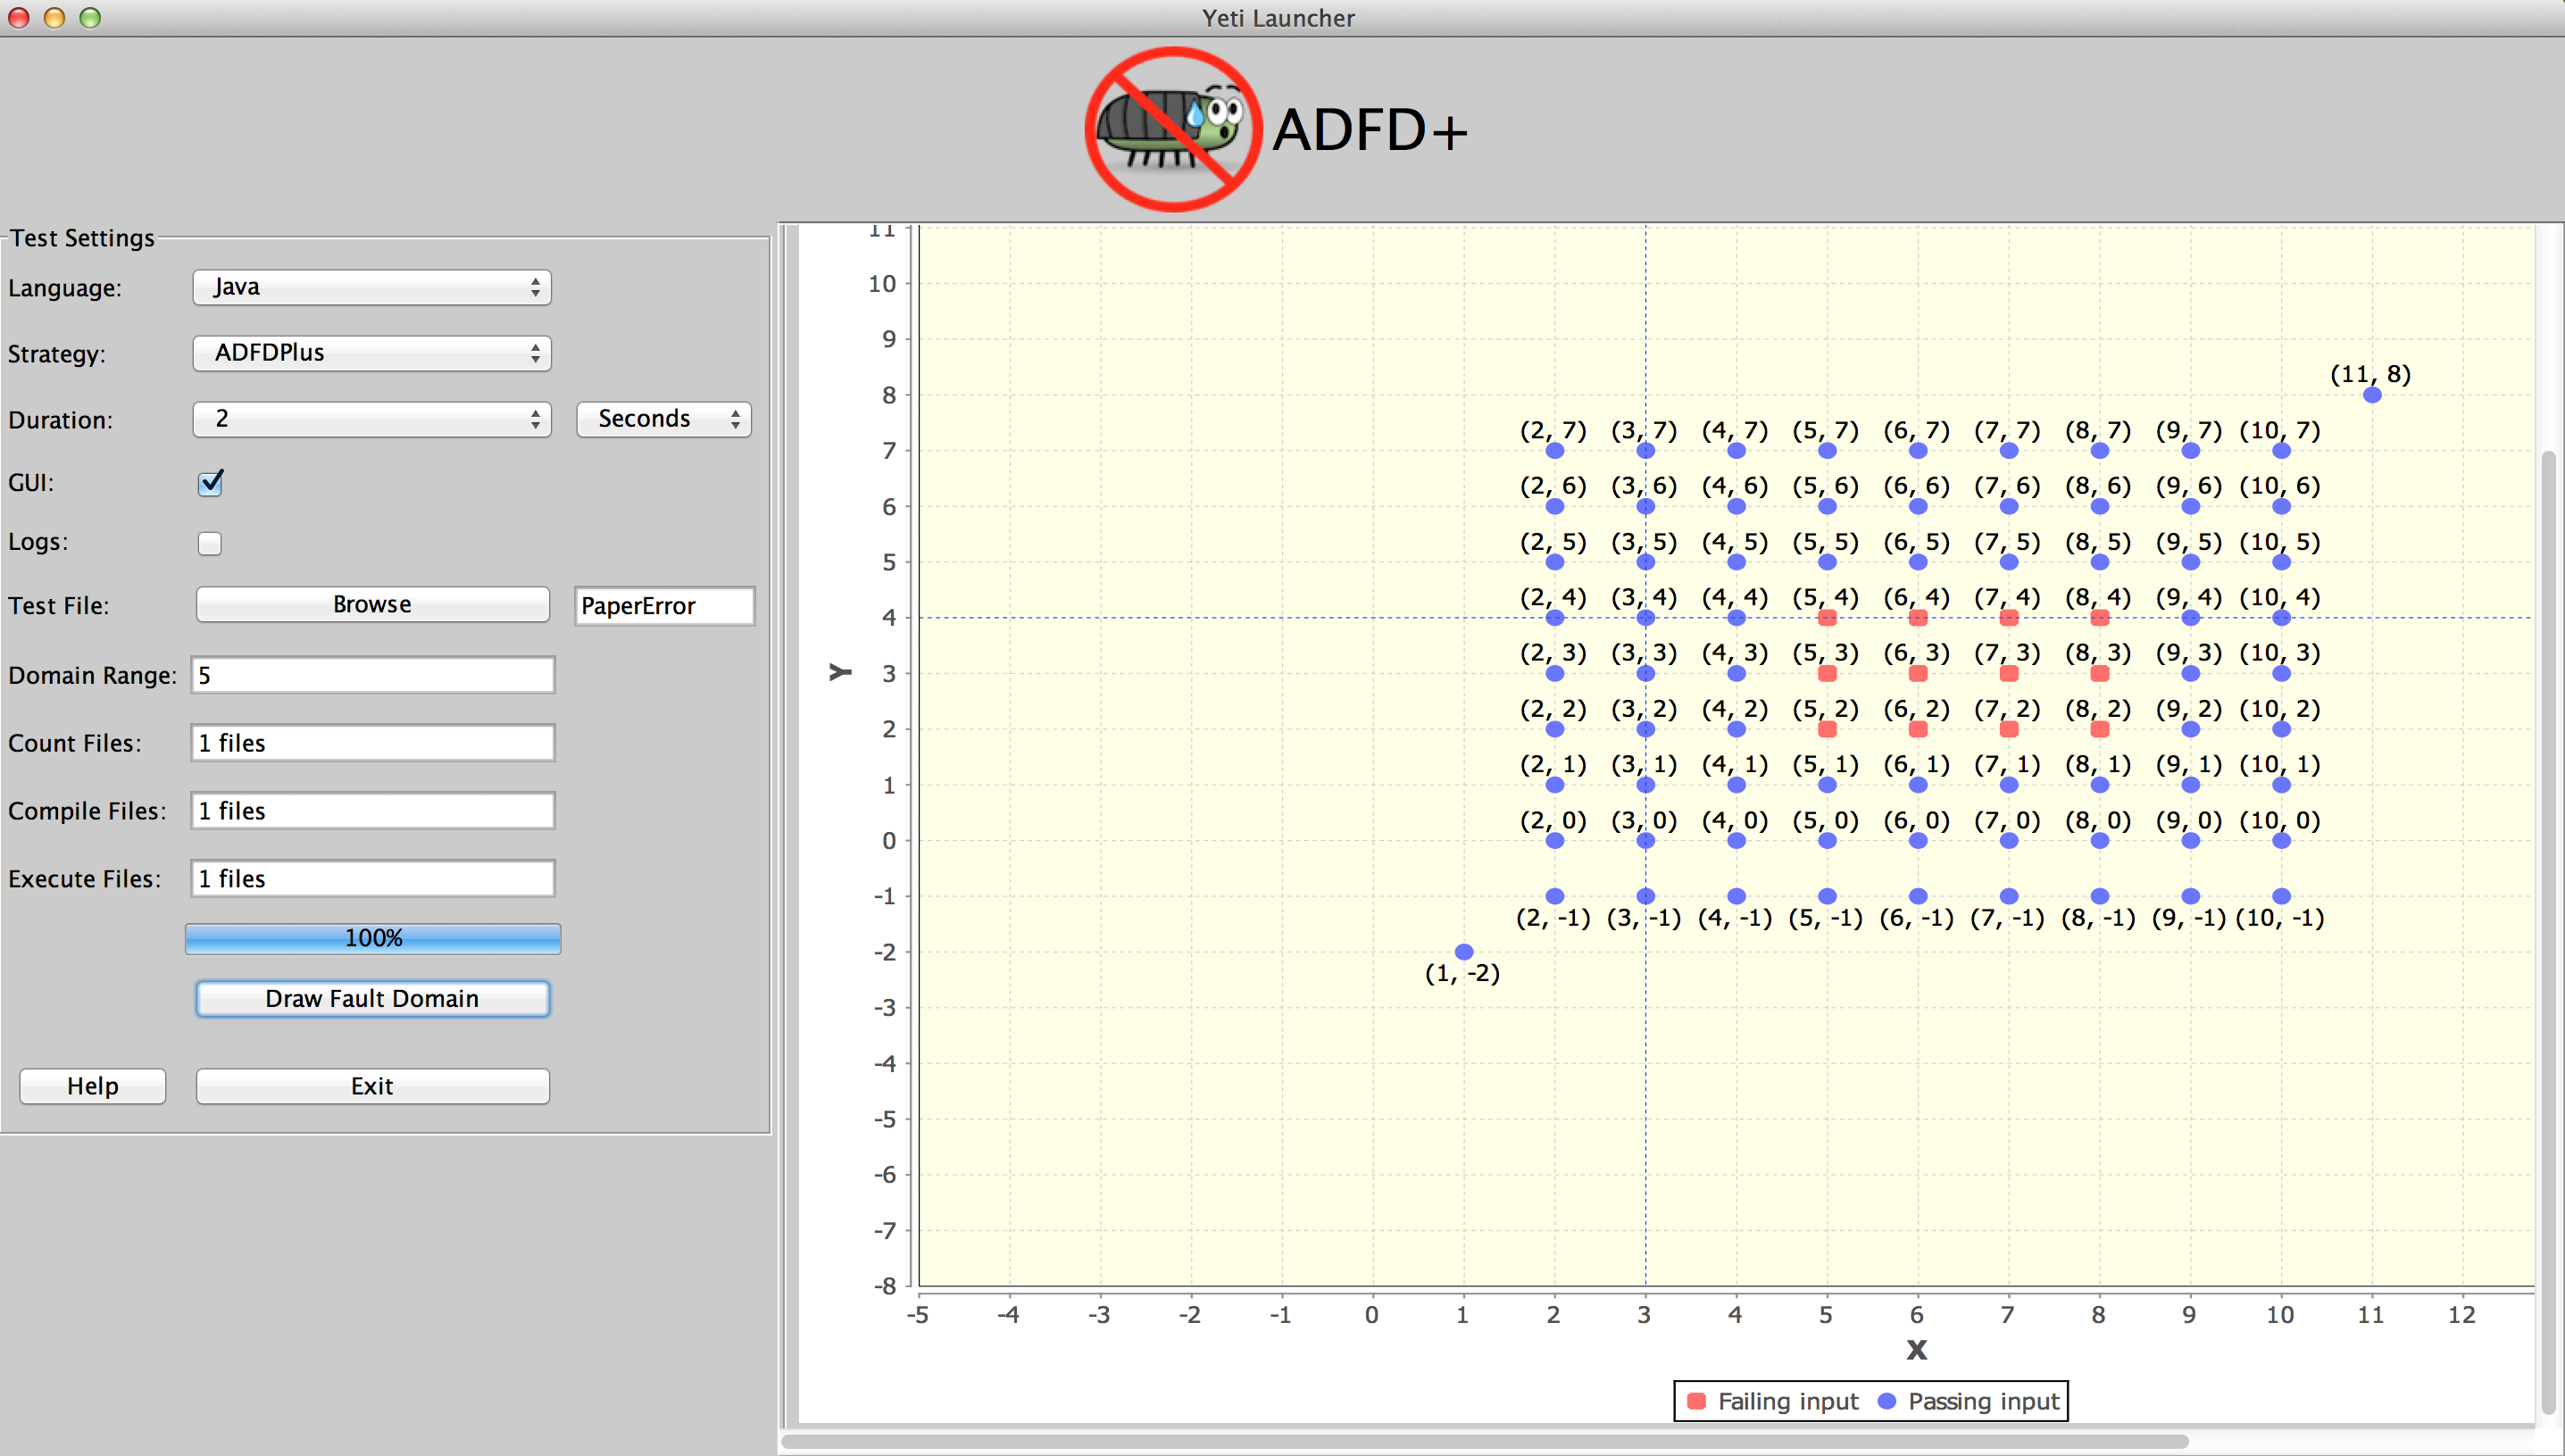
\includegraphics[width=17cm,height=10.3cm]{exampleError.png}
%\caption{The output of ADFD+ for the above code.}
%\label{fig:adfdPlusExample}
%\end{figure*}

%\subsection{Example to illustrate working of ADFD+}
%Suppose we have the following error-seeded class under test. It is evident from the program code that an $ArithmeticException$ (divison by zero) failure is generated when the value of variable $x$ ranges between 5 to 8 and the value of variable $y$ between 2 to 4.

%\begin{lstlisting}
%public class Error {
%  public static void Error (int x, int y){
%    int z;
%    if (((x>=5)&&(x<=8))&&((y>=2)&&(y<=4)))
%		 {
%			 z = 50/0;
%		 }
%   } 
%}
%\end{lstlisting}
%At the beginning of the test, ADFD+ strategy evaluates the given class with the help of YETI and finds the first failure at x = 6 and y = 3. Once a failure is identified ADFD+ uses the surrounding values around it to find a failure domain. The radius of surrounding values is limited to the value set by the user in the $Domain Range$ variable. When the value of $Domain Range$ is set to 5, ADFD+ evaluates a total of 83 values of $x$ and $y$ around the found failure. All evaluated $(x, y)$ values are plotted on a two-dimensional graph with red filled circles indicating fail values and blue filled circles indicating pass values. Figure~\ref{fig:adfdPlusExample} shows that the failure domain forms a block pattern and the boundaries of the failure are $(5, 2), (5, 3),(5, 4), (6, 2), (6, 4), (7, 2), (7, 4), (8, 2), (8, 3), (8, 4)$. 





%%%%%%%%%%%%%%%%%%%%%%%%%%%%%%%%%%%%%%%%%%%%%%%%%
%Randoop maintains two sets called \verb+ErrorSeqs+ and \verb+NonErrorSeqs+ to record the feedback. It extends \verb+ErrorSeqs+ set in case of contract or filter violation and \verb+NonErrorSeqs+ set when no violation is recorded in the feedback. The use of this dynamic feedback evaluation at runtime brings an object to an interesting state. On test completion, \verb+ErrorSeqs+ and \verb+NonErrorSeqs+ are produced as JUnit/NUnit test suite. In terms of coverage and number of faults discovered, Randoop implementing FDRT was compared with JCrasher and JavaPathFinder and 14 libraries of both Java and .Net were evaluated~\cite{visser2004test}. The results showed that Randoop achieved more branch coverage and better fault detection than JCrasher. 

%Daikon is a tool~\cite{ernst2007daikon}, which uses machine-learning technique to automatically generate likely invariants of the program written in C, C++, Java and Pearl. Daikon takes the program and a few test cases as input. The test cases may be either generated manually or by an automated tool. Daikon executes the test cases on the program under test and observes the values that the program computes. At the end of the test session it reports the properties that were true for the observed executions. A feature of Daikon facilitate to process the generated invariants to mitigate non-interesting and redundant invariants. Another feature allows to inserts the generated invariants in to the source code as assertions. The report generated by Daikon is useful in understanding program logic, generating invariants, predicting incompatibilities in component integration, automating theorem proving, repairing inconsistencies in data structures and checking the validity of data streams.

%%%%%%%%%%%%%%%%%    EVALUATION   %%%%%%%%%%%%%%%%%%%%
%\section{Comparison of ADFD+ \& Randoop}\label{sec:eval}
%In order to check the effectiveness and efficiency of ADFD+ we compared it with a random testing tool Randoop. Our subject classes for these experiments were the same that were used in evaluation of ADFD \cite{ahmad2013adfd}. We ran ADFD+ and Randoop for 30 times on each error-seeded one and two dimensional numerical programs, measuring its effectiveness by the total number of test cases used to detect all the failures and its efficiency by the CPU time consumed. 

%\subsection{Research questions} \label{sec:questions}
%The following research questions have been addressed in the study:
%\begin{enumerate}
%
%\item If ADFD and ADFD+ techniques capable of correctly identifying and presenting the failure-domains in production software? %The experimental results claiming the correct identification of ADFD and ADFD+ were based on the purpose build error-seeded programs~\cite{}. To answer the question, we applied the two techniques to all the projects of Qualitas Corpus and examined the results.

%\item \textit{If the graph and invariants generated, correctly represent the failure domains?} %Invariants generated by Daikon can identify the start and stop of the failure domain. To answer this question we compared the generated invariants with the source code and the failure-domain presented in graphical form.
%
%
%\item What are the types and frequency of identified failure-domains? %There are strategies~\cite{}.  that exploit the presence of block and strip failure-domain to get better results. Therefore identifying the presence of underlying failure-domains in production software can help in high quality of software testing.  To answer the questions, we reviewed all the classes containing failure-domains manually, automatically and graphically.
%
%\item If the nature of identified failure-domains is simple or complex and does it make any difference in its identification by manual and automated techniques? % An interesting point is to know what failure is responsible for a failure-domain and how difficult it is to identify that failure by manual testing. To answer this question, we studied the test logs and test output of the automated testing and the source code of the program manually to identify the cause and complexity of failures of failure-domains. 

%\item \textit{If the presence of a particular failure-domain can make it easy or hard to find using automated and manual techniques?} 
%Failure-domain can reside in the form of point, block or strip shape in the input domain. To answer this question we analysed the source code of all the programs in which failure-domains were detected.
%

%\item \textit{If the graph generated by ADFD correctly represent the pass and fail domains?} Both the ADFD and ADFD+ techniques generate graphs to represent failure-domains for simplicity. To answer the question we compared the generated graphs with the source code and the invariants generated by Daikon.
%
%\item If obtained results consistent with previous theoretical and practical results presented?  %As per our knowledge, till now no specific study has been conducted to automatically identify the pass and fail domains however it has been claimed by some researchers~\cite{} that there exist more block and strip patterns then the point patterns. 
%

%\end{enumerate}

%\section{Evaluation} \label{sec:evaluation}
 
%All the programs in which failure-domains were identified are presented in Tables~\ref{table:stripDomains, table:pointDomains, table:blockDomains, table:mixDomains}

% Every program was tested independently by ADFD, ADFD+ and manual testing. All the programs in which failure-domains were identified are presented in Table~\ref{}.  Due to the absence of contracts and assertions in the code under test, undeclared exceptions were taken as failures in accordance with the previous studies~\cite{ahmad2013adfd, Oriol2012}.

%\subsection{Randoop} \label{sec:randoop}
%Random tester for object oriented programs (Randoop) is a fully automatic tool, capable of testing Java classes and .Net binaries. It takes as input a set of classes, time limit or number of tests and optionally a set of configuration files to assist testing. Randoop checks for assertion violations, access violations and un-expected program termination in a given class. Its output is a suite of JUnit for Java and NUnit for .Net program. Each unit test in a test suite is a sequence of method calls (hereafter referred as sequence). Randoop builds the sequence incrementally by randomly selecting public methods from the class under test. Arguments for these methods are selected from the pre-defined pool in case of primitive types and as sequence of null values in case of reference type. Randoop uses feedback mechanism to filter out duplicate test cases. 

%The code for the programs under test is given in Appendix~\ref{} while the test details are presented in Table~\ref{table:Results}. 
%Every class was evaluated through $10^5$ calls in each test session of ADFD+.
%\footnote{The total number of tests is equal to $60\times 30\times 3 \times 10^5 = 540\times10^6~tests$.} 











